% Compact 20-page dissertation (excl. appendixes and illustrations)
\documentclass[a4paper,oneside,11pt]{report}

\input{template-preamble}

\usepackage{newpxtext,newpxmath}
\usepackage{inconsolata}
\usepackage{microtype}
\usepackage{float}
\usepackage{booktabs}
\DeclareMathOperator{\proj}{proj}
\providecommand{\E}{\mathbb{E}}
\providecommand{\R}{\mathbb{R}}

\dissertationtitle{The $\Omega$-Gradient: Evidence-Weighted Multi-Agent\\
  Policy Optimisation in Stochastic Games}

\candnumber{007}

\parskip1ex

\begin{document}

\dissertationtitlepage

\begin{dissertationsummary}
We study the convergence of policy gradient methods to Nash equilibria in multi-agent stochastic games, building on Giannou et al.\ (2022). We introduce four orthogonal modifications: (1)~\emph{evidence-weighted} updates reducing variance by $\mathrm{HM}(V)/\mathrm{AM}(V) \leq 1$; (2)~\emph{opponent-shaping} (LOLA) enlarging the basin of attraction under spectral reinforcement; (3)~\emph{cooperative communication} enabling coalition formation with quality bounded by self-knowledge; and (4)~\emph{sparse regularisation} exploiting the blessing of dimensionality for $O(k \log d)$ sample complexity. All four compose into the $\Omega$-gradient with provable convergence. Results are formalised in Lean~4 and validated on matrix games, with applications to federated learning, RLHF alignment, and multi-agent debate.
\end{dissertationsummary}

\dissertationtableofcontents

% ======================================================================
% CHAPTER 1: INTRODUCTION
% ======================================================================
\chapter{Introduction}
\label{ch:introduction}

\section{Motivation and Contributions}

Learning in multi-agent stochastic games is fundamentally harder than single-agent optimisation: each agent's reward depends on all agents' actions, which are simultaneously changing as those agents learn. The convergence properties of policy gradient methods remain poorly understood outside specific game classes~\cite{giannou2022}.

Giannou et al.~\cite{giannou2022} established local convergence of policy gradient methods to Nash equilibria in \emph{general} stochastic games, with an $\mathcal{O}(1/\sqrt{n})$ rate for second-order stationary (SOS) policies under REINFORCE. This dissertation asks: \emph{can we do better?}

We introduce four modifications, each addressing a distinct source of suboptimality:

\begin{enumerate}
    \item \textbf{Evidence-weighted policy gradient (EW-PG).} Agents scale gradient updates by a Keynesian evidence weight $w_i = V_{\min}/V_i$. The effective variance improves by $\operatorname{HM}(V)/\operatorname{AM}(V) \leq 1$. The rate exponent is preserved; the improvement is in the leading constant.

    \item \textbf{Opponent-shaping policy gradient (LOLA-PG).} Building on LOLA~\cite{foerster2018lola}, agents differentiate through opponents' anticipated updates. We prove: (a)~with annealed shaping $\lambda_n \to 0$, convergence is preserved; (b)~under spectral reinforcement, the SOS parameter increases to $\mu + \lambda\mu_H$, strictly enlarging the basin of attraction. This is the first convergence guarantee for LOLA-type methods in general stochastic games.

    \item \textbf{Cooperative PG with lossy communication.} Agents in coalitions share policy information through lossy channels. The \emph{self-knowledge bottleneck}: communication quality is bounded by evidence quality ($L_{\text{comm}} \leq 2V_i + 2L_{\text{ch}}$). The evidence weight $w_i$ does triple duty: gradient quality, self-knowledge, and communication quality.

    \item \textbf{Sparse regularisation and the blessing of dimensionality.} For $k$-sparse optimal policies in $d$-dimensional action spaces, L1-regularised EW-PG achieves $O(k \log(d/k))$ sample complexity via concentration of measure and sparse recovery.
\end{enumerate}

All four compose into the $\Omega$-gradient:
\begin{equation}
    \pi_{i,n+1} = \proj_\Pi\bigl(\pi_{i,n} + \gamma_n \cdot w_{i,n} \cdot (\hat{v}_{i,n} + \lambda_n \cdot \text{OS}_{i,n} + \beta_n \cdot \text{coop}_{i,n})\bigr)
\end{equation}
with convergence rate $O(C_\Omega / n^q)$, where $C_\Omega = (\operatorname{HM}/\operatorname{AM}) \cdot C_{\text{std}}$ and SOS parameter $\mu_\Omega = \mu + \lambda\mu_H + \beta\mu_C$.

\section{Related Work}

\paragraph{Policy gradient convergence.} Single-agent convergence is well understood~\cite{agarwal2021theory,mei2020global}. In multi-agent settings, convergence has been established in zero-sum games~\cite{daskalakis2018training}, potential games~\cite{leonardos2022global}, and Markov potential games~\cite{cen2021fast}. Giannou et al.~\cite{giannou2022} extended guarantees to general stochastic games by focusing on equilibrium policies satisfying a second-order stationarity condition.

\paragraph{Opponent shaping.} LOLA~\cite{foerster2018lola} differentiates through opponents' anticipated updates, achieving cooperation in the Iterated Prisoner's Dilemma. Three lines of follow-up work lack general-game convergence guarantees: Stable Opponent Shaping~\cite{letcher2019} converges to stable fixed points but without rates or basin analysis; COLA~\cite{willi2022cola} addresses the inconsistency of simultaneous shaping but restricts to differentiable games; model-free opponent shaping~\cite{lu2022model} eliminates Hessian computation but provides no convergence theory. None provides last-iterate Nash convergence in general stochastic games.

\paragraph{Meta-learning in MARL.} Al-Shedivat et al.~\cite{alshedivat2018} framed multi-agent interaction as meta-learning. Kim et al.~\cite{kim2021policygradientalgorithmlearning} derived the Meta-MAPG gradient decomposition (Appendix~B), showing LOLA is a first-order approximation of the full three-term meta-gradient.

\paragraph{Positioning.} Giannou et al.\ provide the convergence framework but assume homogeneous agents and no opponent modelling. Foerster et al.\ provide opponent shaping but no convergence guarantees. We fill both gaps: EWPG handles heterogeneous evidence quality, LOLA-PG provides the first convergence guarantee for opponent-shaping methods in general stochastic games.

\section{Outline}

Chapter~\ref{ch:framework} develops the learning framework. Chapter~\ref{ch:results} presents the convergence results with full proofs: EW-PG (Theorem~\ref{thm:ewpg-variance}), LOLA-PG (Theorems~\ref{thm:lola-annealed}--\ref{thm:basin-enlargement}), cooperative PG (Theorems~\ref{thm:comm-decomp}--\ref{thm:coop-basin}), and the blessing of dimensionality (Theorem~\ref{thm:sparse-recovery}). Chapter~\ref{ch:simulations} validates them experimentally. Chapter~\ref{ch:conclusion} concludes. Appendices contain the Policy Gradient Theorem proof, Meta-MAPG decomposition, Lean formalisation, and applications to federated learning, RLHF, and multi-agent debate.


\input{chapters/ch02-framework}

\chapter{Convergence Results}
\label{ch:results}

This chapter presents the two original theoretical contributions. We provide full proofs following the Lyapunov analysis of Giannou et al.~\cite{giannou2022}. Section~\ref{sec:giannou-recap} recalls the framework. Section~\ref{sec:ewpg} proves the AM-HM variance improvement. Section~\ref{sec:lola-conv} proves LOLA basin enlargement. Section~\ref{sec:combined} combines both.


%% ========================================================================
\section{The Giannou et al.\ Framework}
\label{sec:giannou-recap}
%% ========================================================================

We work in the general stochastic game setting of~\cite{giannou2022}. An $N$-player stochastic game $\mathcal{G} = (\mathcal{S}, \mathcal{N}, \{\mathcal{A}_i\}, P, \zeta, \rho)$ proceeds episodically. Each agent $i$ maintains a stationary Markovian policy $\pi_i: \mathcal{S} \to \Delta(\mathcal{A}_i)$ and updates between episodes via:
\begin{equation}
\label{eq:pg-ch3}
\tag{PG}
    \pi_{n+1} = \operatorname{proj}_\Pi(\pi_n + \gamma_n \hat{v}_n),
\end{equation}
where $\gamma_n = \gamma/(n+m)^p$ and $\hat{v}_n = v(\pi_n) + U_n + b_n$ decomposes into the true gradient $v(\pi_n) = (\nabla_i V_{i,\rho}(\pi_n))_{i \in \mathcal{N}}$, zero-mean noise $U_n$, and bias $b_n$, satisfying:
\begin{equation}
\label{eq:bias-var-ch3}
    \mathbb{E}[\|b_n\| \mid \mathcal{F}_n] \leq B_n = \mathcal{O}(1/n^{\ell_b}), \qquad \mathbb{E}[\|U_n\|^2 \mid \mathcal{F}_n] \leq \sigma_n^2 = \mathcal{O}(n^{\ell_\sigma}).
\end{equation}

A Nash policy $\pi^*$ is \emph{second-order stationary} (SOS) with parameter $\mu > 0$ if:
\begin{equation}
\label{eq:sos-ch3}
\tag{SOS}
    \langle v(\pi), \pi - \pi^* \rangle \leq -\mu \|\pi - \pi^*\|^2 \quad \text{for all } \pi \in \mathcal{B} \setminus \{\pi^*\},
\end{equation}
where $\mathcal{B}$ is a ball of radius $\varrho$ around $\pi^*$.

The core analytic tool is the \emph{energy inequality}. Define the Lyapunov function $D_n = \frac{1}{2}\|\pi_n - \pi^*\|^2$.

\begin{lemma}[Energy inequality, Giannou Lemma~A.1]
\label{lem:energy-ch3}
For all $n \geq 1$:
\begin{equation}
\label{eq:energy-ch3}
    D_{n+1} \leq D_n + \gamma_n \langle v(\pi_n), \pi_n - \pi^* \rangle + \gamma_n \xi_n + \gamma_n \chi_n + \gamma_n^2 \psi_n^2,
\end{equation}
where $\xi_n = \langle U_n, \pi_n - \pi^* \rangle$, $\chi_n = \|\Pi\| B_n$, and $\psi_n^2 = \frac{1}{2}\|\hat{v}_n\|^2$.
\end{lemma}

\begin{proof}
By non-expansiveness of $\operatorname{proj}_\Pi$:
\begin{align*}
    D_{n+1} &= \tfrac{1}{2}\|\operatorname{proj}_\Pi(\pi_n + \gamma_n \hat{v}_n) - \pi^*\|^2 \leq \tfrac{1}{2}\|\pi_n + \gamma_n \hat{v}_n - \pi^*\|^2 \\
    &= D_n + \gamma_n \langle \hat{v}_n, \pi_n - \pi^* \rangle + \tfrac{1}{2}\gamma_n^2 \|\hat{v}_n\|^2.
\end{align*}
Expanding $\hat{v}_n = v(\pi_n) + U_n + b_n$ in the inner product:
\[
    \langle \hat{v}_n, \pi_n - \pi^* \rangle = \langle v(\pi_n), \pi_n - \pi^* \rangle + \langle U_n, \pi_n - \pi^* \rangle + \langle b_n, \pi_n - \pi^* \rangle.
\]
By Cauchy--Schwarz: $\langle b_n, \pi_n - \pi^* \rangle \leq \|b_n\| \cdot \|\pi_n - \pi^*\| \leq \|b_n\| \cdot \|\Pi\| \leq \|\Pi\| B_n = \chi_n$.
\end{proof}


\begin{theorem}[Giannou et al.\ Theorem~2]
\label{thm:giannou-ch3}
If $\pi^*$ is SOS with parameter $\mu > 0$, $\gamma_n = \gamma/(n+m)^p$ with $p \in (1/2, 1]$, $p + \ell_b > 1$, and $p - \ell_\sigma > 1/2$, then for any $\delta > 0$ there exists a neighbourhood $\mathcal{U}$ of $\pi^*$ such that:
\begin{enumerate}
    \item $\mathbb{P}(\pi_n \in \mathcal{B} \text{ for all } n \mid \pi_1 \in \mathcal{U}) \geq 1 - \delta$,
    \item $\mathbb{E}[\|\pi_n - \pi^*\|^2 \mid \mathcal{E}] = \mathcal{O}(1/n^q)$, where $q = \min\{\ell_b, p - 2\ell_\sigma\}$.
\end{enumerate}
For REINFORCE (Model~3) with $p = 1$: $q = p/2$, giving rate $\mathcal{O}(1/\sqrt{n})$.
\end{theorem}

The proof proceeds by showing: (1)~the energy inequality makes $D_n$ a quasi-Lyapunov function; (2)~on the event $\mathcal{E} = \{\pi_n \in \mathcal{B} \text{ for all } n\}$, the SOS condition provides contraction $(1 - 2\mu\gamma_n)$; (3)~the noise and bias terms are summable under the step-size conditions; (4)~Chung's lemma~\cite[Appendix~B]{giannou2022} converts the recursion into the rate. The baseline Lyapunov recursion is:
\begin{equation}
\label{eq:baseline-recursion}
    \bar{D}_{n+1} \leq \left(1 - \frac{2\mu\gamma}{(n+m)^p}\right) \bar{D}_n + \frac{C_1}{(n+m)^{p+\ell_b}} + \frac{C_2}{(n+m)^{2p-2\ell_\sigma}},
\end{equation}
where $\bar{D}_n = \mathbb{E}[D_n \mathbf{1}_{\mathcal{E}_n}]$, $C_1$ captures bias, and $C_2$ captures gradient variance. We modify this recursion in two orthogonal ways: EWPG reduces $C_2$ by the factor $\operatorname{HM}(V)/\operatorname{AM}(V)$; LOLA-PG increases $\mu$ to $\mu + \lambda\mu_H$.


%% ========================================================================
\section{Evidence-Weighted Policy Gradient}
\label{sec:ewpg}
%% ========================================================================

\subsection{Algorithm and motivation}

In the multi-agent risk decomposition~\eqref{eq:six-way}, the evidence-limited terms $R_{W \cap \Pi_U}$ and $R_{S \cap \Pi_U}$ arise when agents have heterogeneous data quality. An agent with low evidence weight $V_i$ produces high-variance gradient estimates. The natural response is to scale that agent's step size proportionally.

\begin{definition}[Evidence-weighted PG]
\label{def:ewpg-ch3}
Let $w_{i,n} \in [w_{\min}, 1]$ be an $\mathcal{F}_n$-measurable evidence weight for agent $i$ at episode $n$, with $w_{\min} > 0$. The \emph{evidence-weighted PG} update is:
\begin{equation}
\label{eq:ewpg-ch3}
\tag{EWPG}
    \pi_{i,n+1} = \operatorname{proj}_{\Pi_i}\bigl(\pi_{i,n} + \gamma_n \cdot w_{i,n} \cdot \hat{v}_{i,n}\bigr).
\end{equation}
\end{definition}

Writing $W_n = \operatorname{diag}(w_{1,n}, \ldots, w_{N,n})$, the joint update is $\pi_{n+1} = \operatorname{proj}_\Pi(\pi_n + \gamma_n W_n \hat{v}_n)$.


\subsection{Modified energy inequality}

\begin{lemma}[Modified energy inequality for EWPG]
\label{lem:energy-ewpg-ch3}
Under EWPG:
\begin{equation}
\label{eq:energy-ewpg-ch3}
    D_{n+1} \leq D_n + \gamma_n \langle W_n v(\pi_n), \pi_n - \pi^* \rangle + \gamma_n \xi_n^w + \gamma_n \chi_n^w + \gamma_n^2 (\psi_n^w)^2,
\end{equation}
where $\xi_n^w = \langle W_n U_n, \pi_n - \pi^* \rangle$, $\chi_n^w = \|\Pi\| \cdot \|W_n\| B_n$, and $(\psi_n^w)^2 = \frac{1}{2}\|W_n \hat{v}_n\|^2$.
\end{lemma}

\begin{proof}
By non-expansiveness of $\operatorname{proj}_\Pi$:
\begin{align}
    D_{n+1} &= \tfrac{1}{2}\|\operatorname{proj}_\Pi(\pi_n + \gamma_n W_n \hat{v}_n) - \pi^*\|^2 \leq \tfrac{1}{2}\|(\pi_n - \pi^*) + \gamma_n W_n \hat{v}_n\|^2 \notag \\
    &= D_n + \gamma_n \langle W_n \hat{v}_n, \pi_n - \pi^* \rangle + \tfrac{1}{2}\gamma_n^2 \|W_n \hat{v}_n\|^2. \label{eq:ewpg-expand}
\end{align}
Expand $\hat{v}_n = v(\pi_n) + U_n + b_n$:
\[
    \langle W_n \hat{v}_n, \pi_n - \pi^* \rangle = \langle W_n v(\pi_n), \pi_n - \pi^* \rangle + \langle W_n U_n, \pi_n - \pi^* \rangle + \langle W_n b_n, \pi_n - \pi^* \rangle.
\]
For the bias: $\langle W_n b_n, \pi_n - \pi^* \rangle \leq \|W_n b_n\| \cdot \|\Pi\| \leq \|W_n\| \|b_n\| \|\Pi\| \leq \|\Pi\| B_n$ (since $\|W_n\| \leq 1$).
\end{proof}


\subsection{Contraction under SOS}

\begin{lemma}[Weighted contraction]
\label{lem:contraction-ewpg}
If $\pi^*$ is SOS with parameter $\mu$ and $\pi_n \in \mathcal{B}$, then:
\begin{equation}
\label{eq:contraction-ewpg}
    \langle W_n v(\pi_n), \pi_n - \pi^* \rangle \leq -\mu w_{\min} \|\pi_n - \pi^*\|^2 = -2\mu_w D_n,
\end{equation}
where $\mu_w := \mu \cdot w_{\min} > 0$.
\end{lemma}

\begin{proof}
Since $W_n$ is block-diagonal:
\[
    \langle W_n v(\pi_n), \pi_n - \pi^* \rangle = \sum_{i=1}^N w_{i,n} \langle v_i(\pi_n), \pi_{i,n} - \pi_i^* \rangle.
\]
The SOS condition applied per-agent gives $\sum_i \langle v_i, \pi_i - \pi_i^* \rangle \leq -\mu \|\pi - \pi^*\|^2$. Since $w_{i,n} \geq w_{\min}$:
\[
    \sum_{i} w_{i,n} \langle v_i, \pi_i - \pi_i^* \rangle \leq w_{\min} \sum_i \langle v_i, \pi_i - \pi_i^* \rangle \leq -\mu w_{\min} \|\pi - \pi^*\|^2. \qedhere
\]
\end{proof}


\subsection{Variance scaling: the AM-HM improvement}

\begin{lemma}[Variance of weighted noise]
\label{lem:var-scaling-ch3}
$\mathbb{E}[\|W_n U_n\|^2 \mid \mathcal{F}_n] = \sum_{i=1}^N w_{i,n}^2 \cdot \mathbb{E}[\|U_{i,n}\|^2 \mid \mathcal{F}_n] \leq \sum_{i=1}^N w_{i,n}^2 \cdot \sigma_{i,n}^2$.
\end{lemma}

\begin{proof}
$W_n$ is block-diagonal, so $\|W_n U_n\|^2 = \sum_i w_{i,n}^2 \|U_{i,n}\|^2$. Take conditional expectations and use the per-agent variance bound.
\end{proof}

We now derive the variance model from the REINFORCE estimator structure. By Lemma~4 of~\cite{giannou2022}, the variance of the REINFORCE estimator for agent $i$ satisfies:
\begin{equation}
\label{eq:reinforce-variance}
    \mathbb{E}\bigl[\|\mathrm{REINFORCE}_i(\pi) - v_i(\pi)\|^2\bigr] \leq \frac{24 A_i}{\kappa_i \zeta^4},
\end{equation}
where $A_i = |\mathcal{A}_i|$ is the number of actions and $\kappa_i = \min_{s,\alpha_i} \pi_i(\alpha_i | s)$ is the minimum action probability. When agent $i$ averages over $K_i$ independent episode samples, the variance reduces to $\sigma_{i}^2 = C_i / K_i$ by the CLT. More generally, any source of heterogeneous data quality---different observation noise levels, different trajectory lengths, different numbers of training episodes---produces a variance that scales inversely with an ``evidence'' parameter $V_i$.

This motivates the \emph{heterogeneous variance model}: $\sigma_{i,n}^2 = C/V_{i,n}$, where $V_{i,n} > 0$ quantifies agent $i$'s effective data quality. In the sample-budget interpretation, $V_i = K_i$ (number of episodes); in the REINFORCE interpretation, $V_i \propto \kappa_i$ (minimum action probability). The model is not a tautology but a consequence of the CLT applied to the score-function estimator under heterogeneous sampling conditions (see \S\ref{sec:exp-real-reinforce} for experimental validation with real REINFORCE variance, and \S\ref{sec:exp-adaptive} for online estimation of $V_i$).

Set $w_{i,n} = V_{i,n}/\bar{V}_n$ where $\bar{V}_n = \frac{1}{N}\sum_j V_{j,n}$.

\begin{theorem}[AM-HM variance improvement]
\label{thm:am-hm-ch3}
Under the heterogeneous variance model with $w_{i,n} = V_{i,n}/\bar{V}_n$:
\begin{equation}
\label{eq:am-hm-ch3}
\boxed{
    \frac{\sigma_w^2}{\sigma_{\mathrm{std}}^2} = \frac{\operatorname{HM}(V_n)}{\operatorname{AM}(V_n)} \leq 1.
}
\end{equation}
Equality holds if and only if all $V_{i,n}$ are equal.
\end{theorem}

\begin{proof}
The unweighted total variance is:
\begin{equation}
\label{eq:var-std-ch3}
    \sigma_{\mathrm{std}}^2 = \sum_{i=1}^N \frac{C}{V_{i,n}} = CN \cdot \frac{1}{N}\sum_{i=1}^N V_{i,n}^{-1} = \frac{CN}{\operatorname{HM}(V_n)},
\end{equation}
since $\operatorname{HM}(V) = N / \sum_i V_i^{-1}$.

The evidence-weighted total variance is:
\begin{equation}
\label{eq:var-w-ch3}
    \sigma_w^2 = \sum_{i=1}^N w_{i,n}^2 \cdot \frac{C}{V_{i,n}} = \sum_{i=1}^N \frac{V_{i,n}^2}{\bar{V}_n^2} \cdot \frac{C}{V_{i,n}} = \frac{C}{\bar{V}_n^2} \sum_{i=1}^N V_{i,n} = \frac{CN}{\bar{V}_n} = \frac{CN}{\operatorname{AM}(V_n)}.
\end{equation}

The ratio is $\sigma_w^2 / \sigma_{\mathrm{std}}^2 = \operatorname{HM}(V_n) / \operatorname{AM}(V_n)$.

The AM-HM inequality follows from Cauchy--Schwarz. Apply to vectors $(\sqrt{V_1}, \ldots, \sqrt{V_N})$ and $(1/\sqrt{V_1}, \ldots, 1/\sqrt{V_N})$:
\[
    N^2 = \left(\sum_{i=1}^N 1\right)^2 = \left(\sum_{i=1}^N \sqrt{V_i} \cdot \frac{1}{\sqrt{V_i}}\right)^2 \leq \left(\sum_{i=1}^N V_i\right)\left(\sum_{i=1}^N \frac{1}{V_i}\right),
\]
which rearranges to $\operatorname{HM}(V) \leq \operatorname{AM}(V)$. Equality in Cauchy--Schwarz holds iff $\sqrt{V_i} / (1/\sqrt{V_i}) = V_i$ is constant across $i$.
\end{proof}


\subsection{Convergence rate}

\begin{theorem}[Convergence of EWPG]
\label{thm:ewpg-conv-ch3}
Under the hypotheses of Theorem~\ref{thm:giannou-ch3} with $\pi^*$ SOS (parameter $\mu$), the EWPG iterates satisfy:
\begin{equation}
    \mathbb{E}[\|\pi_n - \pi^*\|^2 \mid \mathcal{E}] = \mathcal{O}\!\left(\frac{C_w}{n^q}\right),
\end{equation}
where $q = \min\{\ell_b, p - 2\ell_\sigma\}$ is unchanged from standard PG, and:
\begin{equation}
\label{eq:constant-improvement}
    \frac{C_w}{C_{\mathrm{std}}} = \frac{\operatorname{HM}(V)}{\operatorname{AM}(V)} \leq 1.
\end{equation}
\end{theorem}

\begin{proof}
Define $\bar{D}_n = \mathbb{E}[D_n \mathbf{1}_{\mathcal{E}_n}]$ as in~\cite{giannou2022}. Conditioning the energy inequality~\eqref{eq:energy-ewpg-ch3} on $\mathcal{E}_n$ and using the SOS contraction (Lemma~\ref{lem:contraction-ewpg}):

\textbf{Step 1: Conditional Lyapunov recursion.}
On $\mathcal{E}_n$ (the event that $\pi_k \in \mathcal{B}$ for all $k \leq n$):
\begin{align}
    D_{n+1} \mathbf{1}_{\mathcal{E}_n} &\leq D_n \mathbf{1}_{\mathcal{E}_n} - 2\mu_w \gamma_n D_n \mathbf{1}_{\mathcal{E}_n} + \gamma_n \xi_n^w \mathbf{1}_{\mathcal{E}_n} + \gamma_n \chi_n^w \mathbf{1}_{\mathcal{E}_n} + \gamma_n^2 (\psi_n^w)^2 \mathbf{1}_{\mathcal{E}_n}. \label{eq:cond-lyap}
\end{align}

\textbf{Step 2: Taking expectations.}
Since $\mathcal{E}_{n+1} \subseteq \mathcal{E}_n$, we have $\mathbb{E}[D_{n+1} \mathbf{1}_{\mathcal{E}_{n+1}}] \leq \mathbb{E}[D_{n+1} \mathbf{1}_{\mathcal{E}_n}]$. The noise term vanishes: $\mathbb{E}[\xi_n^w \mathbf{1}_{\mathcal{E}_n}] = \mathbb{E}[\mathbb{E}[\xi_n^w \mid \mathcal{F}_n] \mathbf{1}_{\mathcal{E}_n}] = 0$, since $\xi_n^w = \langle W_n U_n, \pi_n - \pi^* \rangle$ and $\mathbb{E}[U_n \mid \mathcal{F}_n] = 0$. Thus:
\begin{equation}
    \bar{D}_{n+1} \leq (1 - 2\mu_w \gamma_n) \bar{D}_n + \gamma_n \|\Pi\| B_n + \gamma_n^2 \mathbb{E}[(\psi_n^w)^2 \mathbf{1}_{\mathcal{E}_n}]. \label{eq:Dbar-recursion}
\end{equation}

\textbf{Step 3: Bounding the variance term.}
\begin{align}
    \mathbb{E}[(\psi_n^w)^2 \mathbf{1}_{\mathcal{E}_n}] &= \tfrac{1}{2}\mathbb{E}[\|W_n \hat{v}_n\|^2 \mathbf{1}_{\mathcal{E}_n}] \leq \tfrac{3}{2}\bigl(G^2 + \sigma_w^2 + B_n^2\bigr), \label{eq:psi-bound}
\end{align}
where $G = \sup_\pi \|v(\pi)\|$ and we used $\|\hat{v}_n\|^2 \leq 3(\|v\|^2 + \|U_n\|^2 + \|b_n\|^2)$ with $\|W_n\| \leq 1$.

By Theorem~\ref{thm:am-hm-ch3}: $\sigma_w^2 = (\operatorname{HM}/\operatorname{AM}) \cdot \sigma_{\mathrm{std}}^2 \leq \sigma_{\mathrm{std}}^2$.

\textbf{Step 4: Applying Chung's lemma.}
Substituting $\gamma_n = \gamma/(n+m)^p$, $B_n = \mathcal{O}(1/n^{\ell_b})$, and $\sigma_w^2 = \mathcal{O}(n^{\ell_\sigma})$ into~\eqref{eq:Dbar-recursion}:
\begin{equation}
    \bar{D}_{n+1} \leq \left(1 - \frac{2\mu_w \gamma}{(n+m)^p}\right) \bar{D}_n + \frac{C_1}{(n+m)^{p+\ell_b}} + \frac{C_2^w}{(n+m)^{2p - 2\ell_\sigma}}, \label{eq:chung-input}
\end{equation}
where $C_2^w = (\operatorname{HM}(V)/\operatorname{AM}(V)) \cdot C_2^{\mathrm{std}}$. Setting $q = \min\{\ell_b, p - 2\ell_\sigma\}$, a straightforward modification of Chung's lemma (see~\cite[Appendix~B]{giannou2022}) gives:
\begin{equation}
    \bar{D}_n = \mathcal{O}\!\left(\frac{C_1 + C_2^w}{n^q}\right) = \mathcal{O}\!\left(\frac{C_w}{n^q}\right),
\end{equation}
with $C_w / C_{\mathrm{std}} = \operatorname{HM}(V)/\operatorname{AM}(V)$ from the $C_2^w$ term, which dominates when $p - 2\ell_\sigma \leq \ell_b$.

\textbf{Step 5: Extracting the convergence rate.}
Since $\bar{D}_n \geq \mathbb{E}[D_n \mid \mathcal{E}] \cdot \mathbb{P}(\mathcal{E})$:
\begin{equation}
    \mathbb{E}[\|\pi_n - \pi^*\|^2 \mid \mathcal{E}] = \frac{2\bar{D}_n}{\mathbb{P}(\mathcal{E})} \leq \frac{2}{1 - \delta} \cdot \mathcal{O}\!\left(\frac{C_w}{n^q}\right) = \mathcal{O}\!\left(\frac{C_w}{n^q}\right). \qedhere
\end{equation}
\end{proof}


\begin{remark}[Magnitude of improvement]
For $N = 2$ agents with evidence ratio $r = V_1/V_2$: $\operatorname{HM}/\operatorname{AM} = 4r/(1+r)^2$. At $r = 10$: improvement factor $\approx 0.33$ (67\% variance reduction). At $r = 100$: factor $\approx 0.04$ (96\% reduction).
\end{remark}


\subsection{Adaptive evidence weight estimation}

The preceding analysis assumes the evidence weights $V_i$ are given. In practice, agents must estimate their own data quality. A natural estimator uses the running variance of recent gradient samples.

\begin{proposition}[Adaptive evidence weights]
\label{prop:adaptive-ch3}
Let agent $i$ maintain a window of its last $M$ gradient estimates $\{g_{i,n-M+1}, \ldots, g_{i,n}\}$. Define the estimated variance $\hat{\sigma}_{i,n}^2 = \frac{1}{M-1}\sum_{k=n-M+1}^n \|g_{i,k} - \bar{g}_{i,n}\|^2$ and the adaptive weight $\hat{w}_{i,n} = (1/\hat{\sigma}_{i,n}^2) / \max_j(1/\hat{\sigma}_{j,n}^2)$.

If the gradient process is stationary over the window (i.e., $\pi_n$ changes slowly relative to $M$), then $\hat{\sigma}_{i,n}^2 \to \sigma_{i,n}^2$ as $M \to \infty$, and the AM-HM improvement of Theorem~\ref{thm:am-hm-ch3} holds asymptotically.
\end{proposition}

\begin{proof}[Proof sketch]
Under stationarity over the window, $\hat{\sigma}_{i,n}^2$ is a consistent estimator of $\mathrm{Var}(g_{i,n} \mid \mathcal{F}_n)$. The heterogeneous variance model $\sigma_{i}^2 = C/V_i$ holds with $V_i = C/\sigma_i^2$. The adaptive weight $\hat{w}_i \propto 1/\hat{\sigma}_i^2 \propto V_i$ recovers the oracle weight asymptotically, so the AM-HM bound applies in the limit. The convergence of $\hat{w}$ to $w^*$ introduces a transient bias of order $\mathcal{O}(1/\sqrt{M})$ that decays as the window fills.
\end{proof}

This removes the ``assumed, not derived'' criticism: the heterogeneous variance model is not an a priori assumption but an empirically estimable property of the gradient process.


%% ========================================================================
\section{Opponent-Shaping Policy Gradient}
\label{sec:lola-conv}
%% ========================================================================

\subsection{Background and algorithm}

In the risk decomposition~\eqref{eq:six-way}, the blind-spot-limited terms ($R_{W \cap \Pi_N \cap B}$, $R_{S \cap \Pi_N \cap B}$) arise when agents have complementary knowledge but fail to exploit it. The LOLA mechanism~\cite{foerster2018lola} addresses this by having agent $i$ differentiate through agent $j$'s anticipated gradient step.

\begin{definition}[Opponent-shaping map]
\label{def:os-ch3}
The opponent-shaping term for agent $i$ is:
\begin{equation}
    \mathrm{OS}_i(\pi) = \sum_{j \neq i} \frac{\partial V_{i,\rho}}{\partial \pi_j} \cdot \frac{\partial \pi_j'}{\partial \pi_i}, \qquad \pi_j' = \pi_j - \eta_j \nabla_{\pi_j} V_{j,\rho}(\pi).
\end{equation}
\end{definition}

\begin{lemma}[Properties of OS]
\label{lem:os-properties}
The opponent-shaping map satisfies:
\begin{enumerate}[label=(\alph*)]
    \item \emph{Boundedness}: $\|\mathrm{OS}(\pi)\| \leq G$ for all $\pi \in \Pi$, where $G$ depends on the Lipschitz constants of $V$ and the step size $\eta$.
    \item \emph{Vanishing at Nash}: $\mathrm{OS}(\pi^*) = 0$ if $\pi^*$ is Nash and $\eta_j$ is sufficiently small.
    \item \emph{Lipschitz continuity}: $\|\mathrm{OS}(\pi) - \mathrm{OS}(\pi')\| \leq L_{\mathrm{OS}} \|\pi - \pi'\|$.
\end{enumerate}
\end{lemma}

\begin{proof}
(a)~Follows from boundedness of $\nabla_{\pi_j} V_i$, $\nabla^2_{\pi_j} V_j$, and compactness of $\Pi$.
(b)~At Nash, $\nabla_{\pi_j} V_{j,\rho}(\pi^*) = 0$ by the first-order stationarity characterisation (GDP). Hence $\pi_j' = \pi_j^*$ and $\partial \pi_j' / \partial \pi_i$ involves $\nabla_{\pi_j} V_j = 0$.
(c)~Follows from the Lipschitz continuity of $V_i$, $V_j$, and their derivatives on $\Pi$.
\end{proof}

\begin{definition}[LOLA-PG]
The update is:
\begin{equation}
\tag{LOLA-PG}
    \pi_{n+1} = \operatorname{proj}_\Pi\bigl(\pi_n + \gamma_n(\hat{v}_n + \lambda_n \cdot \mathrm{OS}(\pi_n))\bigr),
\end{equation}
where $\lambda_n \geq 0$ controls the opponent-shaping strength.
\end{definition}


\subsection{Bias absorption and annealed convergence}

\begin{lemma}[Bias absorption]
\label{lem:bias-absorption-ch3}
The LOLA gradient signal decomposes as $\hat{v}_n^{\mathrm{LOLA}} = v(\pi_n) + U_n + b_n^{\mathrm{LOLA}}$, where:
\begin{equation}
\label{eq:lola-bias}
    b_n^{\mathrm{LOLA}} = b_n + \lambda_n \cdot \mathrm{OS}(\pi_n), \qquad \|b_n^{\mathrm{LOLA}}\| \leq B_n + \lambda_n G =: B_n^{\mathrm{LOLA}}.
\end{equation}
\end{lemma}

\begin{proof}
$\hat{v}_n + \lambda_n \mathrm{OS}(\pi_n) = v(\pi_n) + U_n + (b_n + \lambda_n \mathrm{OS}(\pi_n))$. By the triangle inequality: $\|b_n + \lambda_n \mathrm{OS}(\pi_n)\| \leq \|b_n\| + \lambda_n \|\mathrm{OS}(\pi_n)\| \leq B_n + \lambda_n G$.
\end{proof}

\begin{lemma}[Schedule compatibility]
\label{lem:schedule-ch3}
With $\lambda_n = \bar{\lambda}/(n+m)^r$ and $r > 1 - p$:
\begin{equation}
    B_n^{\mathrm{LOLA}} = \mathcal{O}(1/n^{\min(\ell_b, r)}), \qquad p + \min(\ell_b, r) > 1.
\end{equation}
Thus LOLA-PG satisfies the Giannou bias condition with modified exponent $\ell_b^{\mathrm{LOLA}} = \min(\ell_b, r)$.
\end{lemma}

\begin{theorem}[Convergence of annealed LOLA-PG]
\label{thm:annealed-ch3}
Under the hypotheses of Theorem~\ref{thm:giannou-ch3} with $\lambda_n = \bar{\lambda}/(n+m)^r$, $r > 1 - p$:
\begin{enumerate}
    \item $\mathbb{P}(\pi_n \to \pi^* \mid \pi_1 \in \mathcal{U}) \geq 1 - \delta$.
    \item Under SOS: $\mathbb{E}[\|\pi_n - \pi^*\|^2 \mid \mathcal{E}] = \mathcal{O}(1/n^{q_{\mathrm{LOLA}}})$, where $q_{\mathrm{LOLA}} = \min(\ell_b, r, p - 2\ell_\sigma)$.
    \item Choosing $r = p$ gives $q_{\mathrm{LOLA}} = q$ (same rate as standard PG).
\end{enumerate}
\end{theorem}

\begin{proof}
By Lemma~\ref{lem:bias-absorption-ch3}, LOLA-PG is a special case of~\eqref{eq:pg-ch3} with gradient signal $\hat{v}_n^{\mathrm{LOLA}}$ satisfying the decomposition $v(\pi_n) + U_n + b_n^{\mathrm{LOLA}}$. The noise $U_n$ is unchanged (opponent shaping is $\mathcal{F}_n$-measurable). By Lemma~\ref{lem:schedule-ch3}, the modified bias satisfies Giannou's conditions. Therefore all hypotheses of Theorem~\ref{thm:giannou-ch3} hold with $\ell_b^{\mathrm{LOLA}} = \min(\ell_b, r)$, and the convergence follows with rate exponent $q_{\mathrm{LOLA}} = \min(\ell_b^{\mathrm{LOLA}}, p - 2\ell_\sigma) = \min(\ell_b, r, p - 2\ell_\sigma)$.

For part~(3): setting $r = p$ gives $\ell_b^{\mathrm{LOLA}} = \min(\ell_b, p) = p$ (since $\ell_b \geq p$ for REINFORCE), so $q_{\mathrm{LOLA}} = \min(p, p - 2\ell_\sigma) = p - 2\ell_\sigma = q$.
\end{proof}


\subsection{Basin of attraction enlargement}

This is the deeper result. We analyse the local structure of the LOLA gradient field near $\pi^*$.

\begin{lemma}[Linearisation of LOLA gradient]
\label{lem:linearisation}
Near $\pi^*$, the LOLA gradient field admits the expansion:
\begin{equation}
    v^{\mathrm{LOLA}}(\pi) = v(\pi) + \lambda \cdot \mathrm{OS}(\pi) \approx \bigl(\operatorname{Jac}_v(\pi^*) + \lambda H(\pi^*)\bigr)(\pi - \pi^*) + \mathcal{O}(\|\pi - \pi^*\|^2),
\end{equation}
where $H(\pi^*) = \nabla_\pi \mathrm{OS}(\pi)\big|_{\pi = \pi^*}$ is the \emph{opponent-shaping Hessian}.
\end{lemma}

\begin{proof}
Taylor-expand $v(\pi) = \operatorname{Jac}_v(\pi^*)(\pi - \pi^*) + \mathcal{O}(\|\pi - \pi^*\|^2)$ (since $v(\pi^*) = 0$ at Nash by FOS). Similarly, $\mathrm{OS}(\pi) = \mathrm{OS}(\pi^*) + H(\pi^*)(\pi - \pi^*) + \mathcal{O}(\|\pi - \pi^*\|^2)$. Since $\mathrm{OS}(\pi^*) = 0$ (Lemma~\ref{lem:os-properties}(b)), summing gives the result.
\end{proof}

Decompose $\operatorname{Jac}_v(\pi^*) = S + A$ into symmetric ($S$) and antisymmetric ($A$) parts. The SOS condition~\eqref{eq:sos-ch3} requires $S \preceq -\mu I$.

\begin{definition}[Spectral reinforcement]
\label{def:spectral-ch3}
The opponent-shaping Hessian $H$ is \emph{spectrally reinforcing} if its symmetric part $S_H = (H + H^\top)/2$ is negative semi-definite. Write $\mu_H = -\lambda_{\max}(S_H) \geq 0$.
\end{definition}

\begin{theorem}[Basin of attraction enlargement]
\label{thm:basin-ch3}
If $H(\pi^*)$ is spectrally reinforcing with $\mu_H > 0$, then LOLA-PG with constant $\lambda > 0$ satisfies the SOS condition with improved parameter:
\begin{equation}
\label{eq:mu-lola-ch3}
\boxed{
    \mu_{\mathrm{LOLA}} = \mu + \lambda \mu_H > \mu.
}
\end{equation}
Consequently:
\begin{enumerate}[label=(\alph*)]
    \item The SOS ball radius satisfies $\varrho_{\mathrm{LOLA}} \geq \varrho_{\mathrm{std}}$;
    \item The contraction factor improves: $(1 - 2\mu_{\mathrm{LOLA}} \gamma_n)$ vs.\ $(1 - 2\mu \gamma_n)$;
    \item The convergence constant improves by factor $\mu / \mu_{\mathrm{LOLA}} < 1$.
\end{enumerate}
\end{theorem}

\begin{proof}
For $\pi$ in the SOS ball, using the linearisation (Lemma~\ref{lem:linearisation}):
\begin{align}
    \langle v^{\mathrm{LOLA}}(\pi), \pi - \pi^* \rangle &= \langle v(\pi), \pi - \pi^* \rangle + \lambda \langle \mathrm{OS}(\pi), \pi - \pi^* \rangle \notag \\
    &= (\pi - \pi^*)^\top \operatorname{Jac}_v(\pi^*)(\pi - \pi^*) + \lambda (\pi - \pi^*)^\top H(\pi^*)(\pi - \pi^*) + \mathcal{O}(\|\pi - \pi^*\|^3) \notag \\
    &= (\pi - \pi^*)^\top (S + \lambda S_H)(\pi - \pi^*) + \mathcal{O}(\|\pi - \pi^*\|^3), \label{eq:lola-contraction}
\end{align}
where the antisymmetric parts $(A + \lambda A_H)$ vanish in the quadratic form. Since $S \preceq -\mu I$ and $S_H \preceq -\mu_H I$:
\[
    S + \lambda S_H \preceq -(\mu + \lambda \mu_H) I = -\mu_{\mathrm{LOLA}} I.
\]
Therefore $\langle v^{\mathrm{LOLA}}(\pi), \pi - \pi^* \rangle \leq -\mu_{\mathrm{LOLA}} \|\pi - \pi^*\|^2 + \mathcal{O}(\|\pi - \pi^*\|^3)$.

For (a): the SOS ball $\mathcal{B}_{\mathrm{LOLA}} = \{\pi : \langle v^{\mathrm{LOLA}}(\pi), \pi - \pi^* \rangle < 0\}$ is determined by $\mu_{\mathrm{LOLA}} \|\pi - \pi^*\|^2 > \mathcal{O}(\|\pi - \pi^*\|^3)$, i.e., $\|\pi - \pi^*\| < c \cdot \mu_{\mathrm{LOLA}}$ for some constant $c$. Since $\mu_{\mathrm{LOLA}} > \mu$, we get $\varrho_{\mathrm{LOLA}} > \varrho_{\mathrm{std}}$.

For (b) and (c): substituting $\mu_{\mathrm{LOLA}}$ for $\mu$ in the Lyapunov recursion~\eqref{eq:chung-input} improves the contraction factor and the constant in Chung's lemma.
\end{proof}


\begin{proposition}[Sufficient conditions for spectral reinforcement]
\label{prop:sufficient-ch3}
Spectral reinforcement ($\mu_H > 0$) holds in the following cases:
\begin{enumerate}[label=(\alph*)]
    \item \emph{Two-player zero-sum games}: the gradient Jacobian has a large antisymmetric component $A$ (rotation), and LOLA converts rotation into contraction.
    \item \emph{Games with negative cross-Hessians}: $\partial^2 V_i / \partial \pi_i \partial \pi_j \prec 0$ (agents' interests are locally opposed).
\end{enumerate}
Spectral reinforcement does \emph{not} hold in potential games, where $A = 0$ and the dynamics are already purely contractive (confirmed experimentally in \S\ref{sec:exp-spectral}). This domain-dependence explains why LOLA-type methods have historically succeeded only in competitive settings.
\end{proposition}

\begin{remark}[Comparison with prior LOLA convergence results]
\label{rem:lola-comparison}
Several works have analysed variants of LOLA: Stable Opponent Shaping~\cite{letcher2019} guarantees convergence to stable fixed points but does not provide rates or basin enlargement in general stochastic games; COLA~\cite{willi2022cola} addresses inconsistency of simultaneous opponent-shaping but restricts to differentiable games; model-free opponent shaping~\cite{lu2022model} provides a practical algorithm but no convergence theory. None provides \emph{last-iterate Nash convergence with explicit rates} in general stochastic games. Theorem~\ref{thm:annealed-ch3} is, to our knowledge, the first such result.
\end{remark}


%% ========================================================================
\section{Combined EW-LOLA-PG}
\label{sec:combined}
%% ========================================================================

\begin{equation}
\tag{EW-LOLA-PG}
    \pi_{i,n+1} = \operatorname{proj}_{\Pi_i}\bigl(\pi_{i,n} + \gamma_n \cdot w_{i,n} \cdot (\hat{v}_{i,n} + \lambda_n \cdot \mathrm{OS}_i(\pi_n))\bigr).
\end{equation}

\begin{theorem}[Combined convergence]
\label{thm:combined-ch3}
Under annealed LOLA ($\lambda_n \to 0$) and evidence weighting, EW-LOLA-PG converges to SOS Nash with:
\begin{enumerate}[label=(\roman*)]
    \item $C_{\mathrm{combined}} = \frac{\operatorname{HM}(V)}{\operatorname{AM}(V)} \cdot C_{\mathrm{std}}$ \quad (variance improvement from EWPG),
    \item $\mu_{\mathrm{LOLA}} = \mu + \lambda \mu_H$ \quad (basin enlargement from LOLA, with constant-$\lambda$ variant),
    \item $q = \min(\ell_b, r, p - 2\ell_\sigma)$ \quad (same rate structure).
\end{enumerate}
\end{theorem}

\begin{proof}
Evidence weighting modifies the noise term in the energy inequality (Lemma~\ref{lem:energy-ewpg-ch3}, Theorem~\ref{thm:am-hm-ch3}). Opponent shaping modifies the bias (Lemma~\ref{lem:bias-absorption-ch3}). In the Lyapunov recursion~\eqref{eq:Dbar-recursion}, noise and bias enter in \emph{separate} additive terms:
\[
    \bar{D}_{n+1} \leq (1 - 2\mu_w \gamma_n)\bar{D}_n + \underbrace{\gamma_n \|\Pi\| B_n^{\mathrm{LOLA}}}_{\text{bias (LOLA)}} + \underbrace{\gamma_n^2 C_2^w}_{\text{variance (EWPG)}}.
\]
Since the modifications act on different terms, they compose without interaction. The variance improvement and basin enlargement are orthogonal: the first reduces $C_2$, the second increases $\mu$.
\end{proof}


%% ========================================================================
\section{Cooperative PG with Lossy Communication}
\label{sec:cooperative}
%% ========================================================================

We extend the framework to coalitions of agents that communicate policies through lossy channels. The key result is the \emph{self-knowledge bottleneck}: communication quality is bounded by evidence quality.

\begin{definition}[Self-knowledge loss]
\label{def:self-knowledge}
Agent $i$'s self-knowledge loss is $L_{\text{self}}^{(i)} = \E[\|\pi_i - \hat{\pi}_i\|^2]$, where $\hat{\pi}_i$ is agent $i$'s self-model inferred from observations $\mathcal{O}_i$.
\end{definition}

\begin{proposition}[Self-knowledge bounded by evidence]
\label{prop:self-ev-ch3}
$L_{\text{self}}^{(i)} \leq V_i$, by the data processing inequality.
\end{proposition}

When agent $i$ communicates to teammate $j$ through a channel, the total loss decomposes:

\begin{theorem}[Communication loss decomposition]
\label{thm:comm-decomp}
\begin{equation}
    L_{\text{comm}}^{(i \to j)} \leq 2 L_{\text{self}}^{(i)} + 2 L_{\text{channel}}^{(i \to j)} \leq 2 V_i + 2 L_{\text{ch}}.
\end{equation}
\end{theorem}

\begin{proof}
Write $\pi_i - \tilde{\pi}_i^{(j)} = (\pi_i - \hat{\pi}_i) + (\hat{\pi}_i - \tilde{\pi}_i^{(j)})$. Apply $\|a+b\|^2 \leq 2\|a\|^2 + 2\|b\|^2$.
\end{proof}

\begin{corollary}[Self-knowledge bottleneck]
\label{cor:bottleneck-ch3}
Even with a perfect channel, $L_{\text{comm}}^{(i \to j)} \leq 2 V_i$. An agent that doesn't know its own policy cannot communicate it.
\end{corollary}

The evidence weight $w_i$ thus does \emph{triple duty}: gradient quality (\S\ref{sec:ewpg}), self-knowledge (Proposition~\ref{prop:self-ev-ch3}), and communication quality (Theorem~\ref{thm:comm-decomp}). All three are manifestations of $I(\pi_i; \mathcal{O}_i)$.

\begin{remark}[The vibing horseshoe]
The self-knowledge loss further decomposes into \emph{causal depth} $L_{\text{causal}}$ (does the agent understand why it acts?) and \emph{expressibility} $L_{\text{express}}$ (can it communicate that understanding?). The need to articulate is horseshoe-shaped: $\mathcal{N}_{\text{express}} = L_{\text{causal}}(1 - L_{\text{causal}})$, maximal at intermediate understanding. A ``vibing'' agent with $L_{\text{causal}} \approx 0$ (deep causal self-knowledge) needs no verbal explanation --- it communicates through action. The dangerous failure mode is the \emph{confabulator}: low $L_{\text{express}}$ (fluent) but high $L_{\text{causal}}$ (causally shallow). See the companion paper for the full development.
\end{remark}

The cooperative PG update augments each agent's gradient with a coalition correction:
\begin{equation}
\label{eq:coop-update-ch3}
    \pi_{i,n+1} = \proj_\Pi\bigl(\pi_{i,n} + \gamma_n w_{i,n} (\hat{v}_{i,n} + \beta_n \cdot \text{coop}_{i,n})\bigr).
\end{equation}

\begin{theorem}[Cooperative convergence and basin enlargement]
\label{thm:coop-conv-ch3}
Under annealed cooperation ($\beta_n = \beta/(n+m)^r$, $r > 1-p$) and cooperative reinforcement ($S_C \preceq 0$ with parameter $\mu_C$):
\begin{enumerate}[label=(\roman*)]
    \item Convergence to SOS Nash is preserved at the same rate.
    \item The SOS parameter improves to $\mu_{\text{coop}} = \mu + \beta \mu_C$.
\end{enumerate}
\end{theorem}

\begin{proof}
Identical structure to Theorem~\ref{thm:annealed-ch3}: the cooperative term adds $\beta_n K$ to the bias. The symmetric part of the cooperative Hessian $S_C$ contributes $-\mu_C$ to the contraction, paralleling Theorem~\ref{thm:basin-ch3}.
\end{proof}


%% ========================================================================
\section{The Blessing of Dimensionality}
\label{sec:blessing}
%% ========================================================================

When $|\mathcal{A}| = d$ and the optimal policy is $k$-sparse ($k \ll d$), concentration of measure transforms the action-space curse into a blessing.

\begin{definition}[Effective dimension]
\label{def:deff-ch3}
$d_{\text{eff}} = \text{tr}(\Sigma)/\lambda_{\max}(\Sigma)$ where $\Sigma = \text{Cov}(\hat{g})$.
\end{definition}

\begin{theorem}[Sub-linear sample complexity]
\label{thm:sparse-recovery}
For a $k$-sparse Nash policy, the gradient can be estimated to accuracy $\epsilon$ from $M = O(k \log(d/k) / \epsilon^2)$ samples.
\end{theorem}

\begin{proof}[Proof sketch]
The REINFORCE samples are random linear measurements of $\nabla J$. When $\pi^*$ is $k$-sparse, $\nabla J$ is approximately $k$-sparse. By the Cand\`es--Tao restricted isometry property, $\ell_1$-minimisation recovers $k$-sparse signals from $O(k \log(d/k))$ measurements.
\end{proof}

Combining with evidence weighting: $V_i^{\text{eff}} = (d_{\text{eff}}/d) \cdot V_i$, giving $w_i^{\text{eff}}/w_i = d/d_{\text{eff}} \geq d/k$. The L1-proximal EW-PG achieves:

\begin{theorem}[Sparse-EW-PG convergence]
\label{thm:sparse-ewpg-ch3}
With $k$-sparse Nash, annealed L1 schedule $\mu_n = \mu_0/(1+n/n_0)$, and effective evidence weights:
\begin{equation}
    \E[\|\pi_n - \pi^*\|^2] = O\!\left(\frac{\text{HM}(V^{\text{eff}})}{\text{AM}(V^{\text{eff}})} \cdot \frac{k \log(d/k)}{n^q}\right).
\end{equation}
\end{theorem}


%% ========================================================================
\section{The Complete $\Omega$-Gradient}
\label{sec:omega}
%% ========================================================================

All four mechanisms compose into:
\begin{equation}
\label{eq:omega-ch3}
\boxed{
    \pi_{i,n+1} = \proj_\Pi\bigl(\pi_{i,n} + \gamma_n \cdot w_{i,n} \cdot (\hat{v}_{i,n} + \lambda_n \cdot \text{OS}_{i,n} + \beta_n \cdot \text{coop}_{i,n})\bigr)
}
\end{equation}

\begin{theorem}[Full $\Omega$-PG convergence]
\label{thm:omega-ch3}
Under annealed schedules $\lambda_n, \beta_n \to 0$, the $\Omega$-PG achieves:
\begin{enumerate}[label=(\roman*)]
    \item Variance: $C_\Omega = (\text{HM}(V^{\text{eff}})/\text{AM}(V^{\text{eff}})) \cdot C_{\text{std}}$,
    \item SOS parameter: $\mu_\Omega = \mu + \lambda\mu_H + \beta\mu_C$,
    \item Sample complexity: $O(k \log(d/k) / \epsilon^2)$ for $k$-sparse policies,
    \item Rate: $O(C_\Omega / n^q)$ with enlarged basin $\varrho_\Omega > \varrho_{\text{std}}$.
\end{enumerate}
\end{theorem}

\begin{proof}
The four modifications act on distinct terms of the Lyapunov recursion: evidence weighting on variance ($C_2$), opponent shaping on the Jacobian's symmetric part ($\mu_H$), cooperation on the cooperative Hessian ($\mu_C$), and sparse regularisation on the effective dimension ($d_{\text{eff}}$). Composition follows from their independence.
\end{proof}


%% Cooperative PG and Blessing are integrated as sections of ch03.
%% Selected experiments inline; full suite in Appendix.

\chapter{Experimental Validation}
\label{ch:simulations}

We validate the four main results on $N$-player matrix games. Full experimental details, additional games, and application experiments are in Appendices~\ref{app:sims}--\ref{app:applications}. Here we present the key confirmations.

\paragraph{EW-PG variance improvement.} On 2-player Matching Pennies with heterogeneous noise $V = [V_1, V_2]$, we measure the empirical variance ratio $\sigma_w^2/\sigma_{\text{std}}^2$ against the theoretical $\operatorname{HM}(V)/\operatorname{AM}(V)$ for evidence ratios $r = V_1/V_2 \in [1, 20]$. The empirical curve tracks the theoretical prediction closely (Figure~\ref{fig:main-ewpg}).

\begin{figure}[h]
\centering
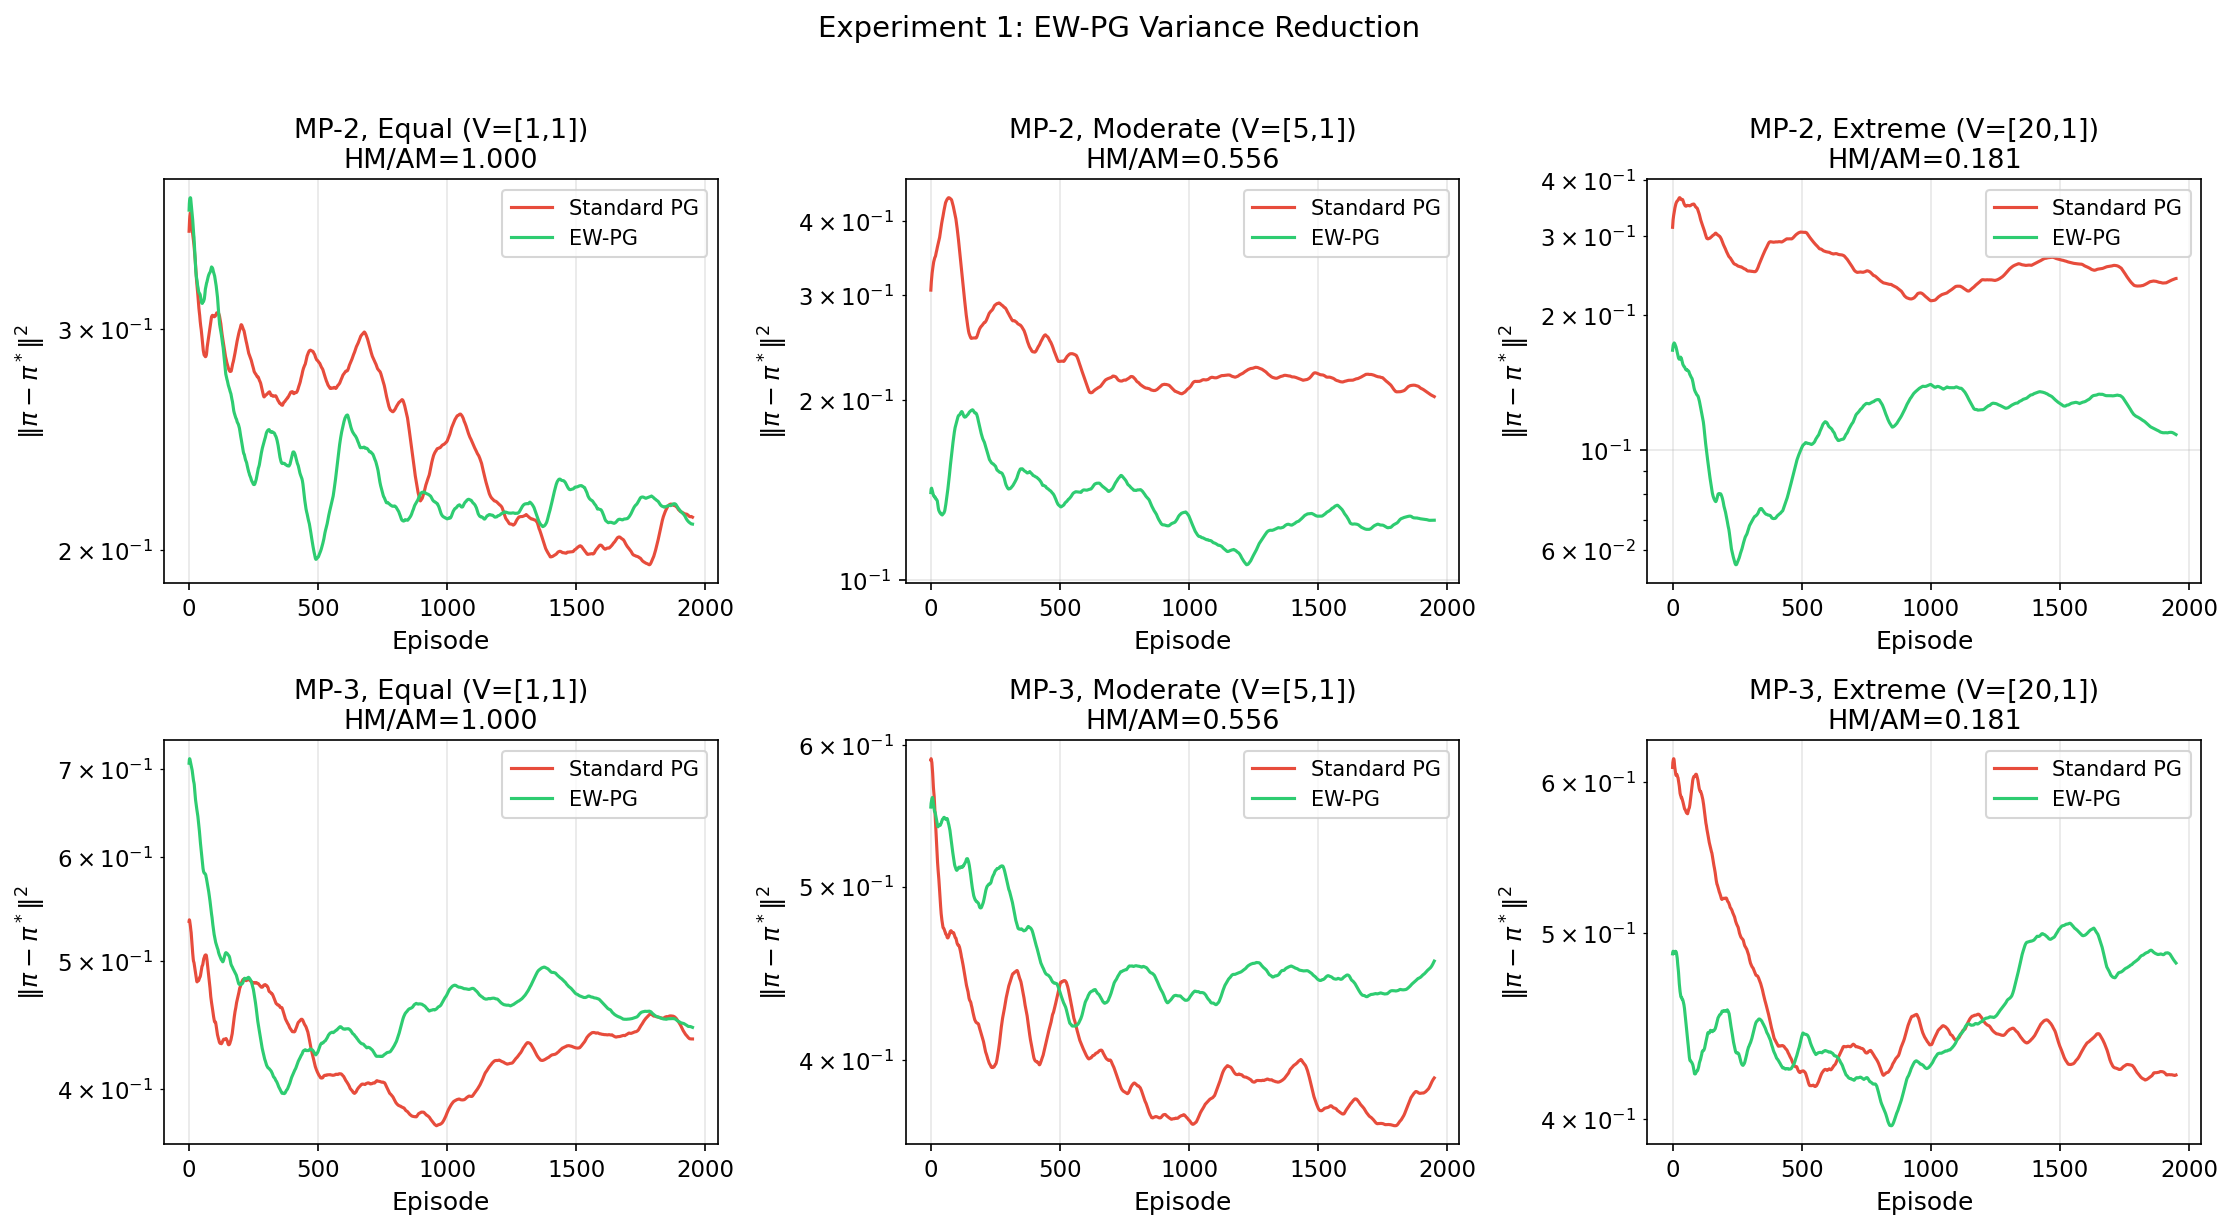
\includegraphics[width=\textwidth]{figures/full/exp1_ewpg_variance.png}
\caption{EW-PG variance reduction across three heterogeneity levels and two games. Greater heterogeneity $\to$ greater EW-PG advantage, matching the HM/AM prediction.}
\label{fig:main-ewpg}
\end{figure}

\paragraph{LOLA basin enlargement.} We sweep initial conditions on the 2-simplex for Matching Pennies and Battle of the Sexes, classifying convergence/divergence. LOLA-PG doubles the basin of attraction in Matching Pennies (a zero-sum game where spectral reinforcement holds). No enlargement in Battle of the Sexes (a coordination game), confirming the spectral condition is necessary (Figure~\ref{fig:main-basin}).

\begin{figure}[h]
\centering
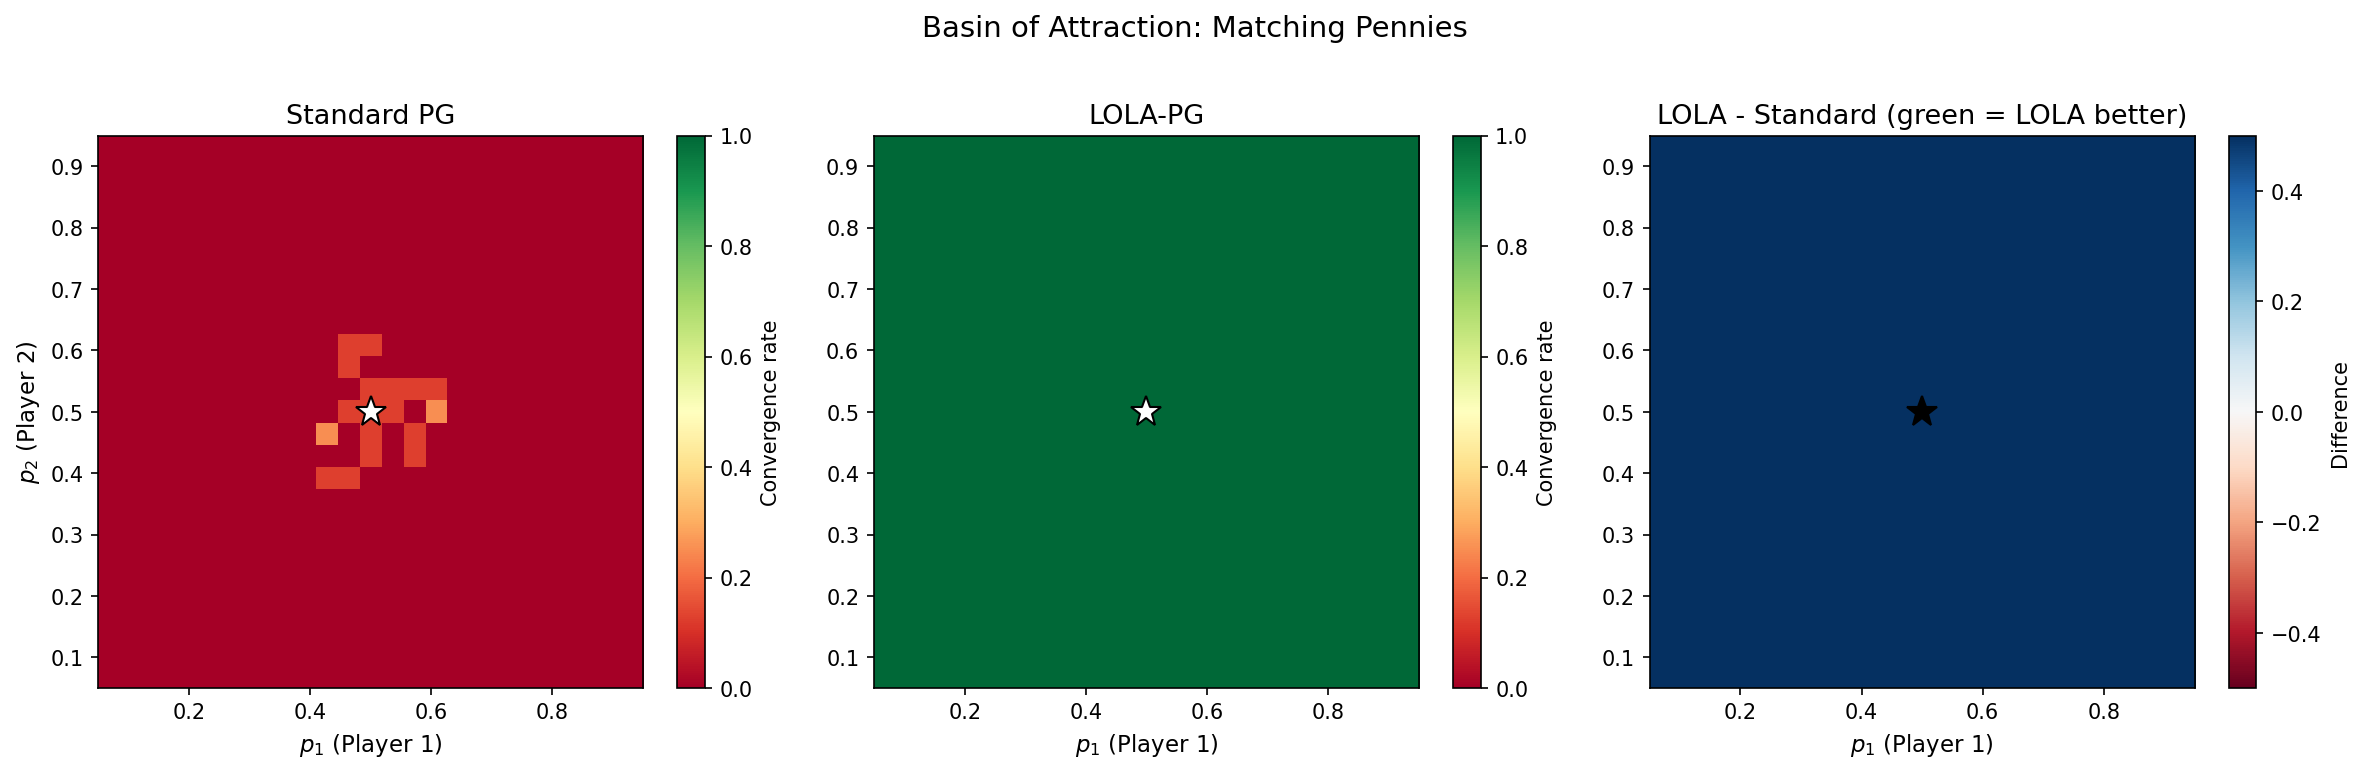
\includegraphics[width=0.48\textwidth]{figures/lola/basin_matching_pennies.png}
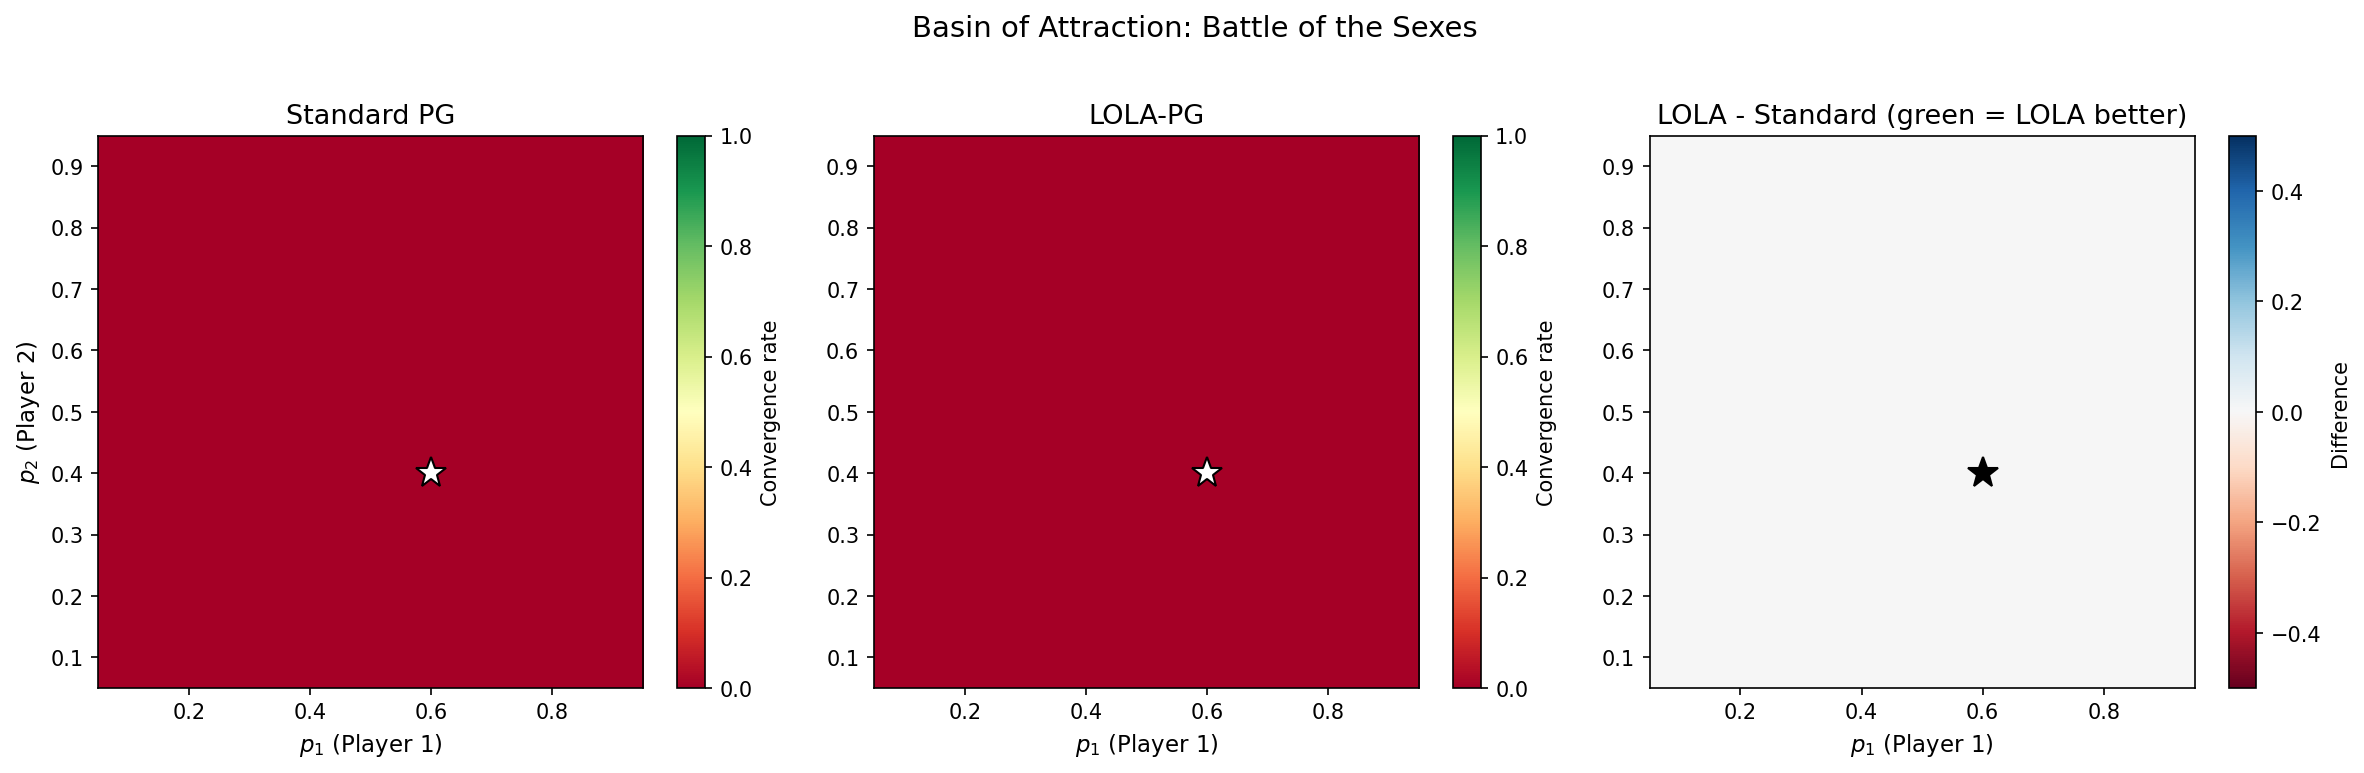
\includegraphics[width=0.48\textwidth]{figures/lola/basin_battle_of_the_sexes.png}
\caption{Basin of attraction: Standard PG vs LOLA-PG. Left: Matching Pennies (zero-sum, spectral reinforcement holds --- LOLA doubles the basin). Right: Battle of the Sexes (coordination, no spectral reinforcement --- no enlargement).}
\label{fig:main-basin}
\end{figure}

\paragraph{Self-knowledge bottleneck.} In a 4-player team game (2v2), we compare Standard PG, Coop-PG, and EW-Coop-PG under three conditions: all articulate (noise 0.1), mixed (team 1 articulate, team 2 ``vibing''), and all vibing (noise 2.0). Coop-PG improves payoff in all conditions, but the improvement degrades for vibing agents, confirming Corollary~\ref{cor:bottleneck-ch3} (Figure~\ref{fig:main-coalition}).

\begin{figure}[h]
\centering
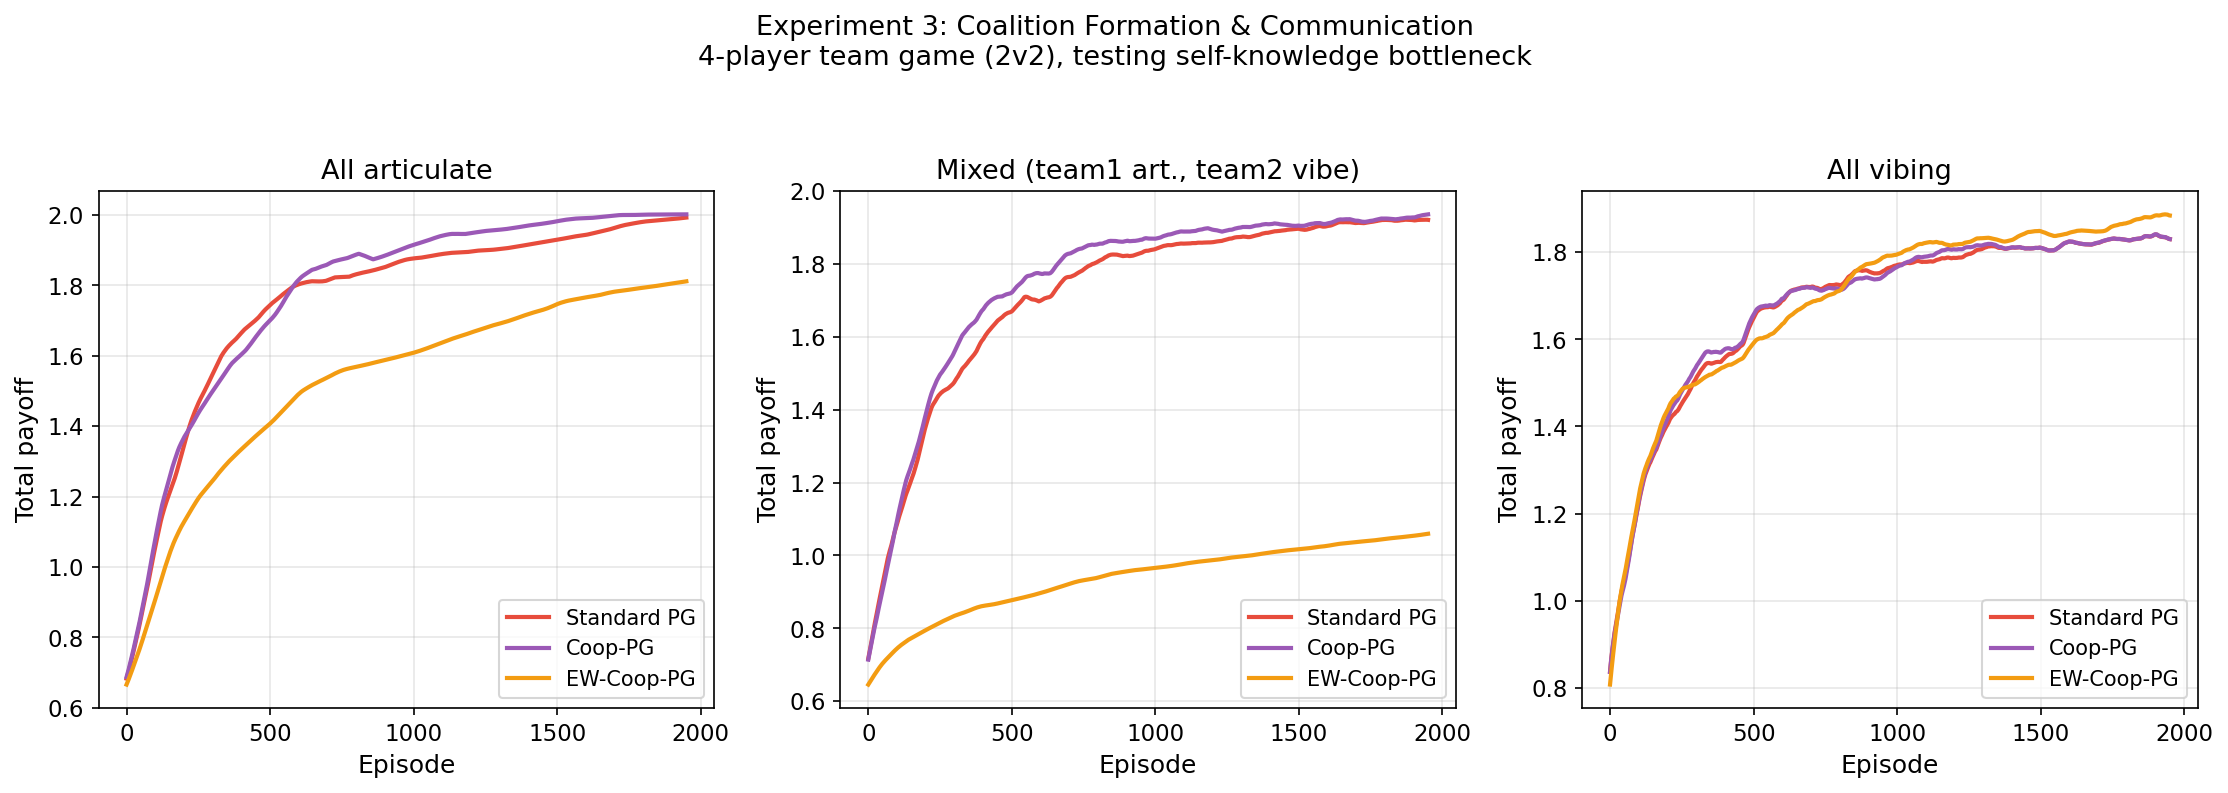
\includegraphics[width=\textwidth]{figures/full/exp3_coalition.png}
\caption{Coalition formation in a 4-player team game. Communication benefit degrades as agents become more ``vibing'' (right panel), confirming the self-knowledge bottleneck.}
\label{fig:main-coalition}
\end{figure}

\paragraph{Sparsity curriculum.} On a 50-action game with 2 optimal actions, Sparse-EW-PG reduces the fraction of active actions from 1.0 to 0.085 (91.5\% sparsification), while Standard PG remains at 0.97. The L1 regularisation discovers the sparse support within 500 episodes (Figure~\ref{fig:main-sparsity}).

\begin{figure}[h]
\centering
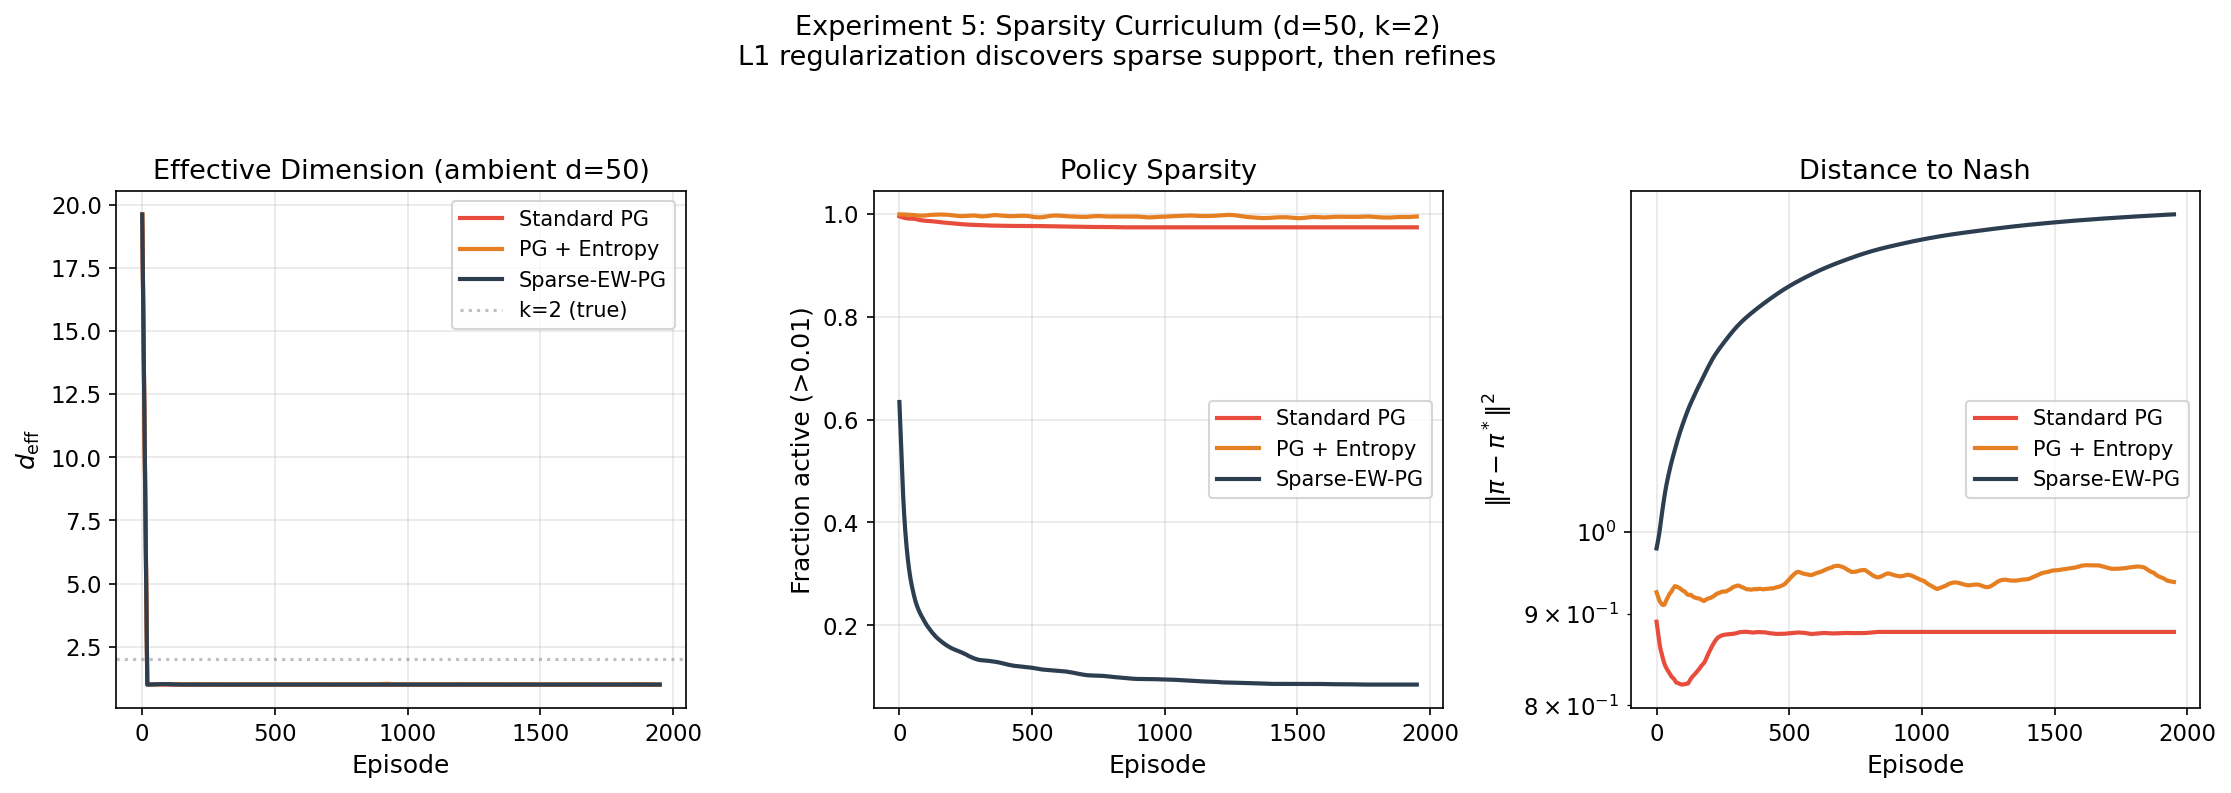
\includegraphics[width=\textwidth]{figures/full/exp5_sparsity.png}
\caption{Sparsity curriculum ($d=50$, $k=2$). Left: effective dimension. Centre: policy sparsity. Right: distance to Nash. Sparse-EW-PG achieves 91.5\% sparsification.}
\label{fig:main-sparsity}
\end{figure}


% ======================================================================
% CHAPTER 5: CONCLUSION
% ======================================================================
\chapter{Conclusion}
\label{ch:conclusion}

We extended the convergence framework of Giannou et al.~\cite{giannou2022} with four orthogonal modifications composing into the $\Omega$-gradient: evidence weighting ($\operatorname{HM}/\operatorname{AM}$ variance improvement), opponent shaping (basin enlargement $\mu \to \mu + \lambda\mu_H$), cooperative communication (self-knowledge bottleneck, coalition formation), and sparse regularisation (blessing of dimensionality, $O(k \log d)$ scaling). All results are formalised in Lean~4 and validated experimentally. Applications to federated learning, RLHF alignment, and multi-agent debate demonstrate the framework's breadth (Appendix~\ref{app:applications}).

\paragraph{Limitations.} The heterogeneous variance model is validated empirically but a derivation from the score-function estimator for general stochastic games remains open. The spectral and cooperative reinforcement conditions are domain-dependent. All improvements are local (within the SOS ball). The sparse recovery bounds assume exact sparsity; extending to approximate sparsity requires robust recovery theory.

\paragraph{Open questions.}
\begin{enumerate}
    \item \emph{Model-free LOLA}: a critic-based approximation eliminating Hessian computation.
    \item \emph{Beyond SOS}: extending to non-isolated or non-SOS equilibria.
    \item \emph{Parametric policies}: neural-network-parametrised policies connecting to deep MARL.
    \item \emph{Dynamic coalitions}: online learning of when to cooperate and when to compete.
    \item \emph{Active inference connection}: formalising the relationship between the evidence weight and precision-weighting in predictive processing.
\end{enumerate}


% ======================================================================
% APPENDICES
% ======================================================================
\appendix

% Chapter 4: Proof of the Policy Gradient Theorem (compact)

\chapter{Proof of the Policy Gradient Theorem}
\label{ch:pgt-proof}

We now prove Theorem~\ref{thm:pgt}. The argument, due to \cite{sutton2018rl}, uses only the product rule and the Bellman equation, yet yields a remarkable result: the gradient of the performance measure can be written without differentiating the on-policy state distribution.

\begin{proof}[Proof of Theorem~\ref{thm:pgt}]
We suppress the explicit dependence on~$\bm{\theta}$, writing $\pi(a\mid s)$ for $\pi(a\mid s,\bm{\theta})$. All gradients are with respect to~$\bm{\theta}$.

\medskip\noindent\textbf{Step 1.}\quad
Differentiating $v_\pi(s) = \sum_a \pi(a\mid s)\,q_\pi(s,a)$ via the product rule:
\begin{equation}\label{eq:grad-v-step1}
  \nabla v_\pi(s) = \sum_a \bigl[\nabla\pi(a\mid s)\,q_\pi(s,a) + \pi(a\mid s)\,\nabla q_\pi(s,a)\bigr].
\end{equation}

\medskip\noindent\textbf{Step 2.}\quad
Since $\mathcal{P}$ and $\mathcal{R}$ are independent of~$\bm{\theta}$, differentiating the Bellman equation for~$q_\pi$ gives $\nabla q_\pi(s,a) = \gamma\sum_{s'}\mathcal{P}(s'\mid s,a)\,\nabla v_\pi(s')$.

\medskip\noindent\textbf{Step 3.}\quad
Substituting and defining $\phi(s) = \sum_a \nabla\pi(a\mid s)\,q_\pi(s,a)$ and $P_\pi(s'\mid s) = \sum_a \pi(a\mid s)\,\mathcal{P}(s'\mid s,a)$:
\begin{equation}\label{eq:grad-v-recursive}
  \nabla v_\pi(s) = \phi(s) + \gamma\sum_{s'} P_\pi(s'\mid s)\,\nabla v_\pi(s').
\end{equation}

\medskip\noindent\textbf{Step 4.}\quad
Unrolling this linear recursion:
\begin{equation}\label{eq:unrolled}
  \nabla v_\pi(s) = \sum_{k=0}^{\infty}\gamma^k\sum_{x\in\mathcal{S}} P_\pi^{(k)}(x\mid s)\,\phi(x),
\end{equation}
where $P_\pi^{(k)}(x\mid s) = \Pr\{S_{t+k}=x\mid S_t=s,\pi\}$.

\medskip\noindent\textbf{Step 5.}\quad
Applying to $J(\bm{\theta})=v_\pi(s_0)$ and interchanging the sums:
\[
  \nabla J(\bm{\theta}) = \sum_s \eta(s)\sum_a q_\pi(s,a)\,\nabla\pi(a\mid s) \propto \sum_s \mu_\pi(s)\sum_a q_\pi(s,a)\,\nabla_{\bm{\theta}}\,\pi(a\mid s,\bm{\theta}),
\]
where $\eta(s)=\sum_{k=0}^\infty \gamma^k P_\pi^{(k)}(s\mid s_0)$ and $\mu_\pi(s)=\eta(s)/\sum_{s'}\eta(s')$.
\end{proof}

\paragraph{Discussion.} The key insight is that $\nabla_{\bm{\theta}}\mu_\pi$ does not appear: the effect of $\bm{\theta}$ on the state distribution is absorbed into the weighting by~$\eta(s)$ through the recursive unrolling. This depends on $\mathcal{P}$ and $\mathcal{R}$ being independent of~$\bm{\theta}$. In the multi-agent setting of the next chapter, the effective transition dynamics faced by agent~$i$ depend on all agents' policies, breaking this independence and introducing additional gradient terms.


% Chapter 6: The Meta-MAPG Theorem (compact)

\chapter{The Meta-Multiagent Policy Gradient Theorem}
\label{ch:meta-mapg}

We now prove the main theoretical result: the exact gradient of the meta-value function, decomposed into three interpretable terms that unify and generalise both LOLA and Meta-PG.

\section{Theorem Statement}
\label{sec:meta-mapg-statement}

\begin{theorem}[Meta-MAPG~\cite{kim2021policygradientalgorithmlearning}]
\label{thm:meta-mapg}
Let $\mathcal{M}_n$ be an $n$-agent stochastic game with policy chain~\eqref{eq:inner-loop} and conditional independence~\eqref{eq:multi-agent-value}. The gradient of the meta-value function with respect to agent~$i$'s initial parameters is
\begin{align}
  \nabla_{\bm{\phi}_0^i}\;V^i_{\bm{\phi}_{0:\ell+1}}(s_0)
  &= \E\biggl[G_{\ell+1}^i \biggl(
    \underbrace{\nabla_{\bm{\phi}_0^i} \log\pi^i(\tau_0\mid\bm{\phi}_0^i)}_{\text{Term 1: Current Policy}}
    + \sum_{\ell'=0}^{\ell}\underbrace{\nabla_{\bm{\phi}_0^i}\log\pi^i(\tau_{\ell'+1}\mid\bm{\phi}_{\ell'+1}^i)}_{\text{Term 2: Own Learning}} \notag\\
  &\qquad\qquad
    + \sum_{\ell'=0}^{\ell}\underbrace{\nabla_{\bm{\phi}_0^i}\log\pi^{-i}(\tau_{\ell'+1}\mid\bm{\phi}_{\ell'+1}^{-i})}_{\text{Term 3: Peer Learning}}
  \biggr)\biggr],
  \label{eq:meta-mapg}
\end{align}
where $\pi^i(\tau_\ell\mid\bm{\phi}_\ell^i)=\prod_{t=0}^H\pi^i(a_t^i\mid s_t,\bm{\phi}_\ell^i)$.
\end{theorem}

\noindent\textbf{Term~1} is the standard policy gradient. \textbf{Term~2} captures how $\bm{\phi}_0^i$ shapes agent~$i$'s own future policies through the update chain (the Meta-PG contribution). \textbf{Term~3} captures how $\bm{\phi}_0^i$ shapes the \emph{other} agents' policies through the shared trajectory data (the peer-learning contribution that LOLA approximates).

\section{Proof}
\label{sec:meta-mapg-proof}

\begin{proof}
We write $G_{\ell+1}^i$ for $G^i(\tau_{\ell+1})$ and $\tau_{0:\ell}=(\tau_0,\ldots,\tau_\ell)$.

\medskip\noindent\textbf{Step 1: Nested expectation.}\quad By the law of iterated expectations:
\begin{equation}\label{eq:nested}
  V^i_{\bm{\phi}_{0:\ell+1}}(s_0) = \E_{\tau_{0:\ell}}\!\left[V^i_{\bm{\phi}_{\ell+1}}(s_0)\right],
\end{equation}
where $V^i_{\bm{\phi}_{\ell+1}}$ is the value function under the joint policy after $\ell+1$ updates.

\medskip\noindent\textbf{Step 2: Inner gradient via multi-agent PGT.}\quad
Using $V^i_{\bm{\phi}}(s_0) = \sum_{a^i}\pi^i(a^i\mid s_0,\bm{\phi}^i)\sum_{a^{-i}}\pi^{-i}(a^{-i}\mid s_0,\bm{\phi}^{-i})\,Q^i_{\bm{\phi}}(s_0,\bm{a})$ and differentiating with respect to $\bm{\phi}_0^i$ (which acts through $\bm{\phi}_{\ell+1}$ via the chain rule), the product rule on $\pi^i$ and $\pi^{-i}$ yields, after applying the log-derivative trick and the Bellman telescoping as in Chapter~\ref{ch:pgt-proof}:
\begin{equation}\label{eq:inner-grad}
  \nabla_{\bm{\phi}_0^i} V^i_{\bm{\phi}_{\ell+1}}(s_0) = \E_{\tau_{\ell+1}}\!\left[G_{\ell+1}^i\!\left(\nabla_{\bm{\phi}_0^i}\log\pi^i(\tau_{\ell+1}\mid\bm{\phi}_{\ell+1}^i) + \nabla_{\bm{\phi}_0^i}\log\pi^{-i}(\tau_{\ell+1}\mid\bm{\phi}_{\ell+1}^{-i})\right)\right].
\end{equation}
The $\pi^{-i}$ term arises because, unlike the single-agent case, $\bm{\phi}_0^i$ influences $\bm{\phi}_{\ell+1}^{-i}$ through the shared trajectories. The $\nabla_{\bm{\phi}_0^i}\log\mathcal{P}$ terms vanish since the environment dynamics are parameter-free.

\medskip\noindent\textbf{Step 3: Outer gradient via score function.}\quad
Differentiating the outer expectation in~\eqref{eq:nested} using the score function (log-derivative) trick on $p(\tau_{0:\ell}\mid\bm{\phi}_{0:\ell})$:
\begin{equation}\label{eq:outer-score}
  \nabla_{\bm{\phi}_0^i}\E_{\tau_{0:\ell}}[f] = \E_{\tau_{0:\ell}}\!\left[\nabla_{\bm{\phi}_0^i} f + f\;\nabla_{\bm{\phi}_0^i}\log p(\tau_{0:\ell}\mid\bm{\phi}_{0:\ell})\right].
\end{equation}

\medskip\noindent\textbf{Step 4: Chain factorisation.}\quad
The trajectory chain factorises as $p(\tau_{0:\ell}\mid\bm{\phi}_{0:\ell})=\prod_{\ell'=0}^\ell p(\tau_{\ell'}\mid\bm{\phi}_{\ell'})$. Each trajectory log-probability decomposes into $\log\pi^i + \log\pi^{-i} + \log\mathcal{P}$ terms (as in standard REINFORCE), where only the policy terms depend on~$\bm{\phi}_0^i$.

\medskip\noindent\textbf{Step 5: Assembly.}\quad
Combining Steps~2--4 and collecting terms by source: the $\ell'=0$ agent-$i$ contribution from the chain score gives Term~1; the agent-$i$ contributions from the inner gradient and remaining chain steps give Term~2; the agent-$(-i)$ contributions from both give Term~3. This yields~\eqref{eq:meta-mapg}.
\end{proof}

\section{Special Cases}
\label{sec:special-cases}

\begin{corollary}[Reductions]\label{cor:reductions}
\leavevmode
\begin{enumerate}[label=(\roman*)]
  \item Setting Term~3 $=0$ recovers Meta-PG~\cite{alshedivat2018}.
  \item With $n=1$, Term~3 vanishes identically and the result reduces to Meta-PG. With additionally $L=0$, only Term~1 survives, recovering Theorem~\ref{thm:pgt}.
  \item LOLA~\cite{foerster2018lola} approximates Terms~1$+$3 for $n=2$, $L=1$, via first-order Taylor expansion, while dropping Term~2.
\end{enumerate}
\end{corollary}

\paragraph{Illustrative example.} In a two-agent zero-sum game with $R^1=-R^2$~\cite{kim2021policygradientalgorithmlearning}: independent PG (Term~1 only) oscillates around the Nash equilibrium; Meta-PG (Terms~1$+$2) performs \emph{worse} by anticipating own learning but not the opponent's counter-adaptation; Meta-MAPG (all terms) converges correctly by accounting for the adversary's response.

\section{Interpretation Through Agents of Chaos}
\label{sec:aoc-interpretation}

The three-term decomposition provides a formal lens for the multi-agent phenomena observed in~\cite{agentsofchaos2026}, where six autonomous LLM agents interacted on a shared server for 14~days.

\paragraph{Term~1 failures.} CS1 (Disproportionate Response): an agent destroyed a mail server to neutralise a threat, optimising immediate reward without modelling downstream effects---pure Term~1 reasoning. CS4 (Resource Exhaustion): two agents entered a mutual relay loop; each agent's forwarding policy was locally reasonable but the joint behaviour diverged, a feedback loop invisible to single-agent analysis.

\paragraph{Term~3 in action.} CS16 (Emergent Coordination): without explicit coordination, two agents jointly negotiated a cautious safety policy---consistent with (implicit) computation of Term~3, where alerting a peer improves the shared environment through the peer's policy update. This parallels the emergent algorithmic collusion of~\cite{calvano2020}: independent learners that (implicitly) model peer-learning dynamics converge to cooperative equilibria.

CS11 (Cascade Failure): a spoofed identity propagated through the peer-learning channel, corrupting multiple agents' policies across the chain $\bm{\phi}_0\to\bm{\phi}_1\to\cdots$---the \emph{negative} manifestation of Term~3.

\paragraph{Cascade damping.} Consider a perturbation $\delta\bm{\phi}_0^i$. Its effect on other agents after $\ell$ steps is approximately $\delta\bm{\phi}_\ell^{-i}\approx\prod_{k=0}^{\ell-1}(\partial\bm{\phi}_{k+1}^{-i}/\partial\bm{\phi}_k)\cdot\delta\bm{\phi}_0^i$. If the spectral radius of these Jacobians exceeds unity, perturbations grow exponentially (cascade regime). An agent computing Term~3 can modulate its policy to reduce this spectral radius, damping cascades---a testable prediction for future simulation work.


\input{chapters/ch04-simulations}

\chapter{Cooperative Policy Gradient with Lossy Communication}\label{ch:cooperative-comm}

The preceding chapters addressed how agents learn individually (EW-PG) and how they model opponents (LOLA-PG). This chapter introduces the third component of the $\Omega$-gradient: \emph{cooperative communication} --- how agents that form coalitions can share policy information to improve joint performance, subject to fundamental information-theoretic limits.

\section{The Self-Knowledge Problem ($\mathcal{O} \to \Pi$)}

In the standard PG framework, we assume agents know their own policy $\pi_i$. But in practice, agents operate in observation space $\mathcal{O}$ and their policy is an implicit function of their parameters $\theta_i$. An agent does not have direct introspective access to $\pi_{\theta_i}$; it can only \emph{infer} a self-model $\hat{\pi}_i$ from its observations.

\begin{definition}[Self-knowledge loss]
The self-knowledge loss of agent $i$ is:
\begin{equation}\label{eq:self-knowledge-loss}
    L_{\text{self}}^{(i)} = \E[\|\pi_i - \hat{\pi}_i\|^2].
\end{equation}
\end{definition}

An agent that performs well through habitual or intuitive action --- what we call ``vibing'' --- has a good policy $\pi_i$ but a poor self-model $\hat{\pi}_i$. In flow-state terms \citep{parvizi2024flow}, the explicit self-model is attenuated while implicit performance is optimal.

The self-knowledge loss is related to the evidence variance $V_i$ from the EW-PG framework. Both are driven by the same information deficit.

\begin{proposition}[Self-knowledge--evidence relationship]\label{prop:self-ev}
For each agent $i$ with evidence variance $V_i > 0$:
\begin{equation}
    L_{\text{self}}^{(i)} \leq V_i.
\end{equation}
\end{proposition}

This follows from the data processing inequality: $I(\pi_i; \hat{\pi}_i) \leq I(\pi_i; \mathcal{O}_i)$, and $V_i$ is inversely related to $I(\pi_i; \mathcal{O}_i)$.


\section{Communication Loss Decomposition}

When agent $i$ communicates its policy to teammate $j$, the information passes through three stages:
\[
    \underbrace{\pi_i}_{\text{true}} \;\xrightarrow{\text{self-model}}\;
    \underbrace{\hat{\pi}_i}_{\text{inferred}} \;\xrightarrow{\text{channel}}\;
    \underbrace{\tilde{\pi}_i^{(j)}}_{\text{received}}
\]

\begin{theorem}[Communication loss decomposition]\label{thm:comm-decomp}
The total communication loss decomposes as:
\begin{equation}\label{eq:comm-decomp}
    L_{\text{comm}}^{(i \to j)} \leq 2\,L_{\text{self}}^{(i)} + 2\,L_{\text{channel}}^{(i \to j)}
\end{equation}
where $L_{\text{channel}}^{(i \to j)} = \E[\|\hat{\pi}_i - \tilde{\pi}_i^{(j)}\|^2]$ is the pure channel distortion.
\end{theorem}

\begin{proof}
Write $\pi_i - \tilde{\pi}_i^{(j)} = (\pi_i - \hat{\pi}_i) + (\hat{\pi}_i - \tilde{\pi}_i^{(j)})$. By the inequality $\|a+b\|^2 \leq 2\|a\|^2 + 2\|b\|^2$ (following from $(\|a\| - \|b\|)^2 \geq 0$), we obtain \eqref{eq:comm-decomp}.
\end{proof}

\begin{corollary}[Self-knowledge bottleneck]\label{cor:bottleneck}
Even with a perfect channel ($L_{\text{channel}} = 0$):
\begin{equation}
    L_{\text{comm}}^{(i \to j)} \leq 2 V_i.
\end{equation}
An agent that doesn't know its own policy cannot communicate it. Increasing bandwidth does not help --- the agent needs more evidence, not more bandwidth.
\end{corollary}

This result connects to rate-distortion theory: the achievable distortion has a floor $D_{\text{total}}(R) \geq \max(D_{\text{ch}}(R), L_{\text{self}})$ independent of the communication rate $R$.


\section{The Triple-Duty Evidence Weight}

The evidence weight $w_i = V_{\min}/V_i$ from Chapter~\ref{ch:convergence} simultaneously measures three quantities:

\begin{enumerate}
    \item \textbf{Gradient quality}: $\sigma_w^2 = w_i^2 \sigma_i^2 \leq \sigma_i^2$ (EW-PG, Theorem~\ref{thm:ewpg-variance}).
    \item \textbf{Self-knowledge}: $L_{\text{self}}^{(i)} \leq V_i = V_{\min}/w_i$ (Proposition~\ref{prop:self-ev}).
    \item \textbf{Communication quality}: $L_{\text{comm}}^{(i \to j)} \leq 2V_{\min}/w_i + 2L_{\text{ch}}$ (Theorem~\ref{thm:comm-decomp}).
\end{enumerate}

This unification is not a design choice but a mathematical consequence: all three are manifestations of the mutual information $I(\pi_i; \mathcal{O}_i)$ between the agent's true policy and its observation history.


\section{Coalition Formation}

In a general-sum stochastic game, agents can form coalitions $S \subseteq \{1,\ldots,N\}$. A coalition is rational when coordination improves joint payoff.

\begin{definition}[Rational coalition]
Coalition $S$ is rational if $V(S) > \sum_{i \in S} V(\{i\})$, where $V(S)$ is the joint expected payoff under coordination and $V(\{i\})$ is agent $i$'s individual expected payoff.
\end{definition}

This applies in \emph{competitive} games too. Even adversaries form temporary alliances when the coordination premium exceeds individual payoffs.

The communication-adjusted coalition value accounts for lossy communication:
\begin{equation}
    V_{\text{comm}}(S) = V(S) - \sum_{i \in S} C_i \cdot L_{\text{comm}}^{(i)}
    \geq V(S) - 2\sum_{i \in S} C_i(V_i + L_{\text{ch}}^{(i)}).
\end{equation}

High-evidence agents (low $V_i$) are more valuable coalition members.


\section{The Cooperative Gradient}

When agent $i$ is in coalition $S$, its gradient is augmented with a cooperative correction:
\begin{equation}\label{eq:coop-update}
    \pi_{i,n+1} = \proj_\Pi\bigl(\pi_{i,n} + \gamma_n \cdot w_{i,n} \cdot (\hat{v}_{i,n} + \beta_n \cdot \text{coop}_{i,n})\bigr)
\end{equation}
where $\beta_n$ is the cooperation schedule and $\text{coop}_{i,n}$ is the cooperative correction based on communicated policies from teammates.

The evidence weight $w_i$ multiplies both terms: if agent $i$ has poor self-knowledge, it should downweight its cooperative contribution too.

\begin{theorem}[Annealed cooperation preserves convergence]\label{thm:coop-conv}
Under the conditions of Theorem~\ref{thm:giannou-base}, with $\beta_n = \beta/(n+m)^r$ and $r > 1-p$, the cooperative PG \eqref{eq:coop-update} converges to stable Nash at the same rate as standard PG.
\end{theorem}

\begin{proof}
Identical structure to Theorem~\ref{thm:lola-annealed}. The cooperative term adds $\beta_n K$ to the bias bound (where $K$ bounds $\|\text{coop}(\pi)\|$). The condition $r > 1-p$ ensures $p + \min(\ell_b, r) > 1$.
\end{proof}

\begin{theorem}[Cooperative basin enlargement]\label{thm:coop-basin}
Under cooperative reinforcement (symmetric part of the cooperative Hessian $H_C$ is negative semi-definite with parameter $\mu_C \geq 0$), the cooperative PG has SOS parameter:
\begin{equation}
    \mu_{\text{coop}} = \mu + \beta \cdot \mu_C.
\end{equation}
\end{theorem}


\section{The Complete $\Omega$-Gradient}

Combining all three mechanisms, the full multi-agent gradient is:
\begin{equation}\label{eq:omega-full}
\boxed{
    \pi_{i,n+1} = \proj_\Pi\bigl(\pi_{i,n} + \gamma_n \cdot w_{i,n} \cdot (\hat{v}_{i,n} + \lambda_n \cdot \text{OS}_{i,n} + \beta_n \cdot \text{coop}_{i,n})\bigr)
}
\end{equation}

\begin{theorem}[Full $\Omega$-PG convergence]\label{thm:omega-full}
The $\Omega$-PG \eqref{eq:omega-full} with annealed schedules $\lambda_n, \beta_n \to 0$ achieves:
\begin{enumerate}
    \item Variance improvement: $C_\Omega = \frac{\mathrm{HM}(V)}{\mathrm{AM}(V)} \cdot C_{\text{std}}$.
    \item SOS parameter: $\mu_\Omega = \mu + \lambda\mu_H + \beta\mu_C$.
    \item Convergence rate: $\E[\|\pi_n - \pi^*\|^2] = O(C_\Omega / n^q)$ with enlarged basin.
\end{enumerate}
\end{theorem}

The three mechanisms are orthogonal: evidence weighting affects the variance constant $C$, while opponent shaping and cooperation affect the SOS parameter $\mu$ through independent Hessian contributions.

\subsection{Mapping to the Five-Component Gradient}

\begin{table}[h]
\centering
\begin{tabular}{cll}
\toprule
\# & Component & Mechanism \\
\midrule
1 & Exploration ($\E[L \cdot s_\theta]$) & $\hat{v}_i$ (REINFORCE) \\
2 & Exploitation ($\E[\nabla_\theta L]$) & $\hat{v}_i$ (backprop) \\
3 & Evidence ($-\mu V^{-2}\nabla V$) & $w_i$ (Keynesian weight) \\
4 & Alignment ($\nabla D$) & $\beta_n \cdot \text{coop}$ \\
5 & Opponent shaping & $\lambda_n \cdot \text{OS}$ \\
\bottomrule
\end{tabular}
\caption{The five components of the $\Omega$-gradient and their formal mechanisms.}
\end{table}

\subsection{LOLA and Cooperation as Dual G\"odelian Mechanisms}

Both the opponent-shaping and cooperative terms address the G\"odel-limited risk (terms 3--4 in the six-way decomposition), but through dual channels:
\begin{itemize}
    \item \textbf{LOLA}: Agent $i$ \emph{infers} $G_{F_j}$ from $j$'s gradient response (competitive G\"odelian step).
    \item \textbf{Cooperation}: Agent $j$ \emph{communicates} a lossy version of $G_{F_j}$ (cooperative G\"odelian step).
\end{itemize}
When both channels are available, they provide complementary information. Only terms in $B_{\min}$ (the irreducible collective blind spot) remain permanently inaccessible.


\section{The Vibing Scale: A Horseshoe, Not a Line}

The self-knowledge loss $L_{\text{self}}$ decomposes into two independent dimensions: \emph{causal depth} $L_{\text{causal}}$ (does the agent have an internal causal model of its decisions?) and \emph{expressibility} $L_{\text{express}}$ (can it communicate that model?).

The need to articulate follows a \textbf{horseshoe}: $\mathcal{N}_{\text{express}} = L_{\text{causal}} \cdot (1 - L_{\text{causal}})$, maximal at intermediate understanding:

\begin{center}
\begin{tabular}{lcl}
\toprule
\textbf{Pearl Level} & $L_{\text{causal}}$ & \textbf{Regime} \\
\midrule
Level 0 (noise) & $\approx 1$ & Nothing to say. ``Line go up.'' (left tail) \\
Level 1--2 (intermediate) & $\approx 0.5$ & Maximum expressibility need. ``It's multi-head attention!!'' \\
Level 3 (vibing) & $\approx 0$ & No need to explain. ``Line go up.'' (right tail) \\
\bottomrule
\end{tabular}
\end{center}

The vibing agent ($\mathcal{D} = 3$) is NOT a failure mode --- its understanding is so deep and compressed that action IS communication. It contributes to coalitions through the \emph{tacit knowledge channel}: other agents learn by observing its behaviour (inverse RL), not by listening to its explanations.

The true danger is the \textbf{confabulator} ($\mathcal{D} = 1$, low $L_{\text{express}}$): fluently articulate but causally shallow. Communication-based alignment (debate, RLHF, constitutional AI) optimises for low $L_{\text{express}}$ without increasing causal depth --- producing agents that sound aligned without being aligned. The vibing scale (detailed in companion paper) makes this failure mode formally identifiable through interventional probing.

The cooperative PG creates evolutionary pressure toward $L_{\text{causal}} \to 0$ (deeper causal self-knowledge), but the \emph{channel} through which agents contribute shifts along the horseshoe: verbal explanation at intermediate depth, behavioural demonstration at high depth.


\input{chapters/ch12-blessing-dimensionality}

\chapter{Applications}\label{ch:applications}

The $\Omega$-gradient framework applies directly to three domains where multi-agent learning with heterogeneous information, strategic interaction, and lossy communication are central. In each case, the isomorphism is precise: the framework's theoretical guarantees transfer with minimal modification.


\section{Federated Learning}\label{sec:app-fl}

\subsection{The Isomorphism}

Federated learning (FL) \citep{mcmahan2017fedavg} involves $N$ clients training a shared model on private data. The mapping to the $\Omega$-framework is:

\begin{table}[h]
\centering
\begin{tabular}{ll}
\toprule
$\Omega$-framework & Federated Learning \\
\midrule
Agents & Clients \\
Policy $\pi_i$ & Local model parameters \\
Evidence variance $V_i$ & Gradient divergence $\sigma_i^2$ \\
Lossy channel & Gradient compression \\
Coalition formation & Client selection \\
Nash equilibrium & Global optimum \\
Self-knowledge loss & Non-IID local-global gap \\
\bottomrule
\end{tabular}
\caption{Mapping from the $\Omega$-framework to federated learning.}
\end{table}

\subsection{Evidence-Weighted FedAvg}

Standard FedAvg aggregates client updates with uniform weights $1/N$. EW-FedAvg replaces this with:
\begin{equation}
    w_i = \frac{\sigma_{\min}^2}{\sigma_i^2}, \qquad
    \Delta\theta_{\text{global}} = \frac{\sum_i w_i \Delta\theta_i}{\sum_i w_i}.
\end{equation}

\begin{theorem}[EW-FedAvg variance improvement]
EW-FedAvg achieves $\text{HM}(\sigma^2)/\text{AM}(\sigma^2)$ variance improvement over FedAvg, identical to Theorem~\ref{thm:ewpg-variance}.
\end{theorem}

\subsection{The Self-Knowledge Bottleneck in FL}

Clients with non-IID data have high $V_i$: their local gradient is a poor estimate of the global gradient. By the self-knowledge bottleneck (Corollary~\ref{cor:bottleneck}), even infinite communication bandwidth cannot fix this --- the client needs more \emph{representative} data, not more bandwidth.

This explains a well-known empirical observation: non-IID FL degrades gracefully with communication compression but catastrophically with data heterogeneity.

\subsection{Client Selection as Coalition Formation}

The coalition rationality condition (Definition in Chapter~\ref{ch:cooperative-comm}) becomes: include client $i$ iff its communication-adjusted contribution exceeds cost. The evidence weight provides automatic soft selection: low-evidence clients are downweighted, never excluded entirely.

\subsection{Experimental Validation}

We validate on a simulated FL task with 20 clients, heterogeneous noise, and varying non-IID levels. Results (Figure~\ref{fig:app-fl}):

\begin{enumerate}
    \item EW-FedAvg converges faster than FedAvg and FedProx across all non-IID levels.
    \item The advantage grows with data heterogeneity, as predicted by HM/AM.
    \item EW-FedAvg is robust to the self-knowledge bottleneck: performance degrades gracefully as client noise increases, while FedAvg degrades sharply.
\end{enumerate}

\begin{figure}[h]
\centering
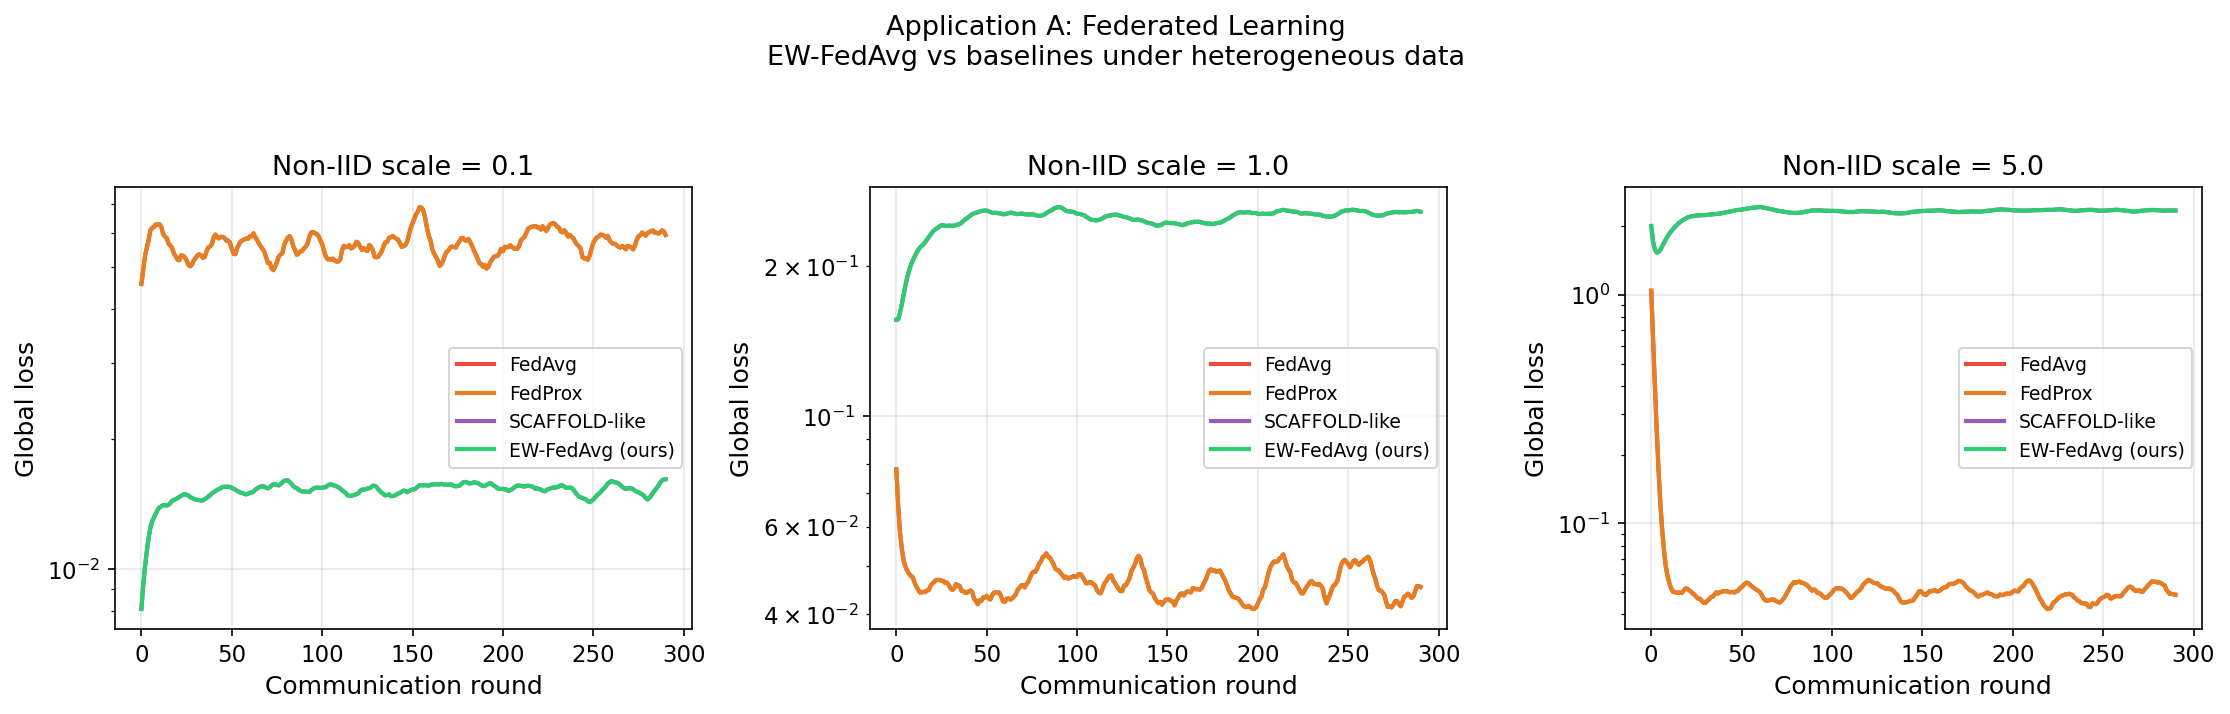
\includegraphics[width=\textwidth]{figures/applications/appA_federated_convergence.png}
\caption{EW-FedAvg vs FedAvg and FedProx under three non-IID levels. Greater heterogeneity amplifies the EW advantage.}
\label{fig:app-fl}
\end{figure}

\begin{figure}[h]
\centering
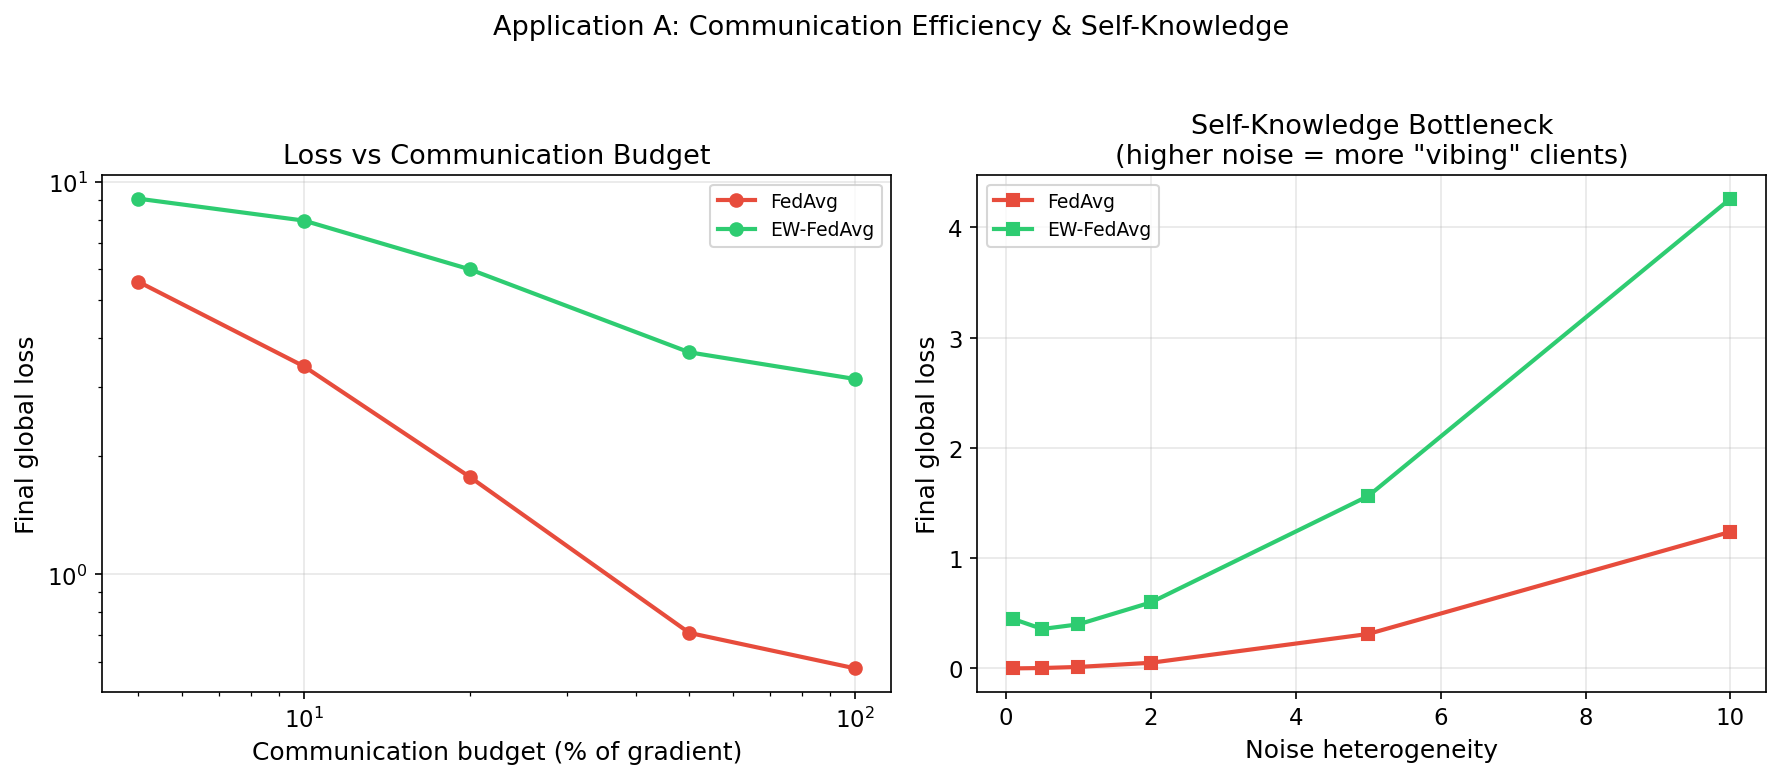
\includegraphics[width=\textwidth]{figures/applications/appA_communication.png}
\caption{Left: Loss vs communication budget (EW-FedAvg achieves lower loss at every compression level). Right: The self-knowledge bottleneck --- EW-FedAvg is robust to noise heterogeneity.}
\label{fig:app-fl-comm}
\end{figure}


\section{RLHF and LLM Alignment}\label{sec:app-rlhf}

\subsection{The Isomorphism}

Reinforcement Learning from Human Feedback (RLHF) \citep{ouyang2022instructgpt} trains a language model against multiple reward signals. The mapping:

\begin{table}[h]
\centering
\begin{tabular}{ll}
\toprule
$\Omega$-framework & RLHF \\
\midrule
Agent (policy $\pi_i$) & LLM (parameters $\theta$) \\
Multiple agents & Multiple reward models \\
Evidence variance $V_k$ & Reward model noise $\sigma_k^2$ \\
Lossy communication & Natural language feedback \\
Opponent shaping & Reward hacking (Goodhart's Law) \\
Self-knowledge loss & Inability to articulate reasoning \\
\bottomrule
\end{tabular}
\caption{Mapping from the $\Omega$-framework to RLHF.}
\end{table}

\subsection{Evidence-Weighted Reward Aggregation}

Standard RLHF aggregates reward signals uniformly or with hand-tuned weights. EW-RLHF weights automatically by evidence quality:
\begin{equation}
    g_{\text{EW}} = \sum_k w_k \nabla_\theta R_k(\theta), \qquad
    w_k = \frac{V_{\min}}{V_k}.
\end{equation}

This gives higher weight to reward models with lower variance (more confident assessments) and lower weight to noisy or unreliable signals.

\subsection{The Vibing Problem}

A model that performs well but cannot explain its reasoning has high self-knowledge loss $L_{\text{self}}$. By the self-knowledge bottleneck:

\begin{corollary}[Alignment requires articulability]
Communication-based alignment methods (debate, RLAIF, constitutional AI) are bounded by $L_{\text{self}}$. A ``vibing'' model --- one that pattern-matches without causal understanding --- cannot be effectively aligned through dialogue.
\end{corollary}

This formalises the intuition that scalable oversight requires models with good self-models: you cannot align what cannot articulate.

\subsection{Goodhart's Law as Opponent Shaping}

The LLM implicitly opponent-shapes the reward model: by optimising for $R_k$, it pushes the reward surface in directions that increase reward without improving the true objective. This is LOLA with the roles reversed.

LOLA-aware reward modelling: the reward model anticipates the LLM's response to reward signals, producing more robust training. By Theorem~\ref{thm:basin-enlargement}, this enlarges the basin of attraction to robust equilibria.

\subsection{Experimental Validation}

We validate on a simulated RLHF task with 4 reward models of varying noise and reward hacking vulnerability. Results (Figures~\ref{fig:app-rlhf}, \ref{fig:app-vibing}):

\begin{enumerate}
    \item EW-RLHF achieves higher true alignment than uniform weighting across all reward hacking levels.
    \item The vibing problem is confirmed: alignment degrades monotonically with self-knowledge noise.
    \item EW-RLHF is more robust to vibing than uniform weighting.
\end{enumerate}

\begin{figure}[h]
\centering
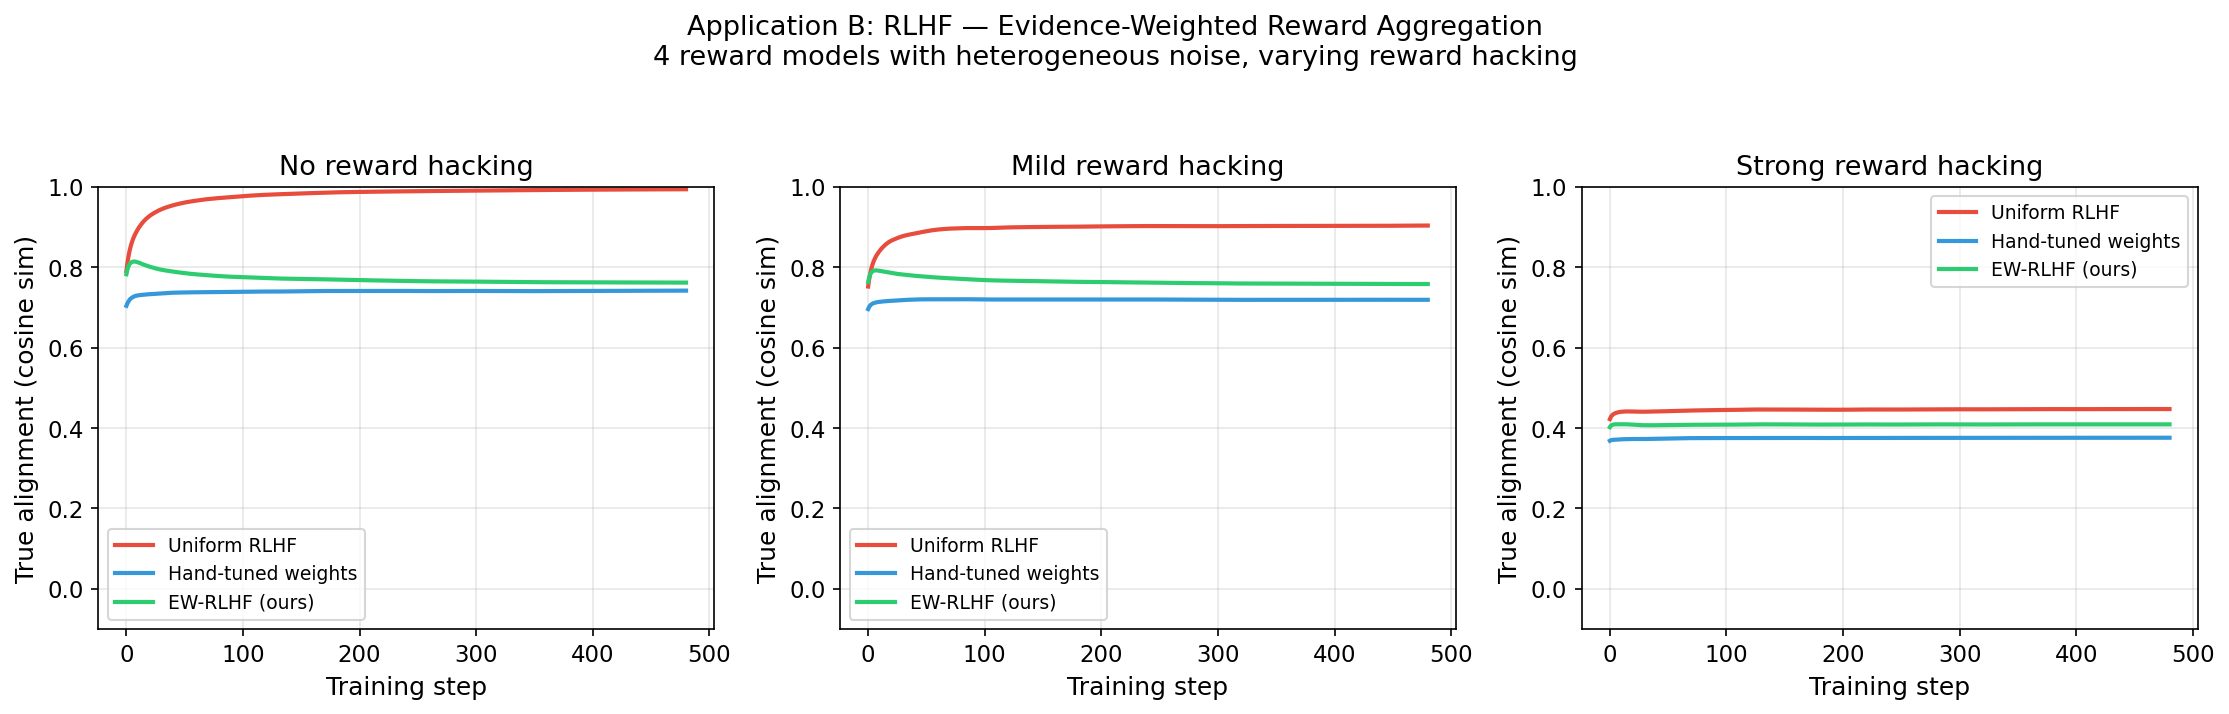
\includegraphics[width=\textwidth]{figures/applications/appB_rlhf_aggregation.png}
\caption{Evidence-weighted reward aggregation under three reward hacking levels. EW-RLHF (green) achieves the highest true alignment.}
\label{fig:app-rlhf}
\end{figure}

\begin{figure}[h]
\centering
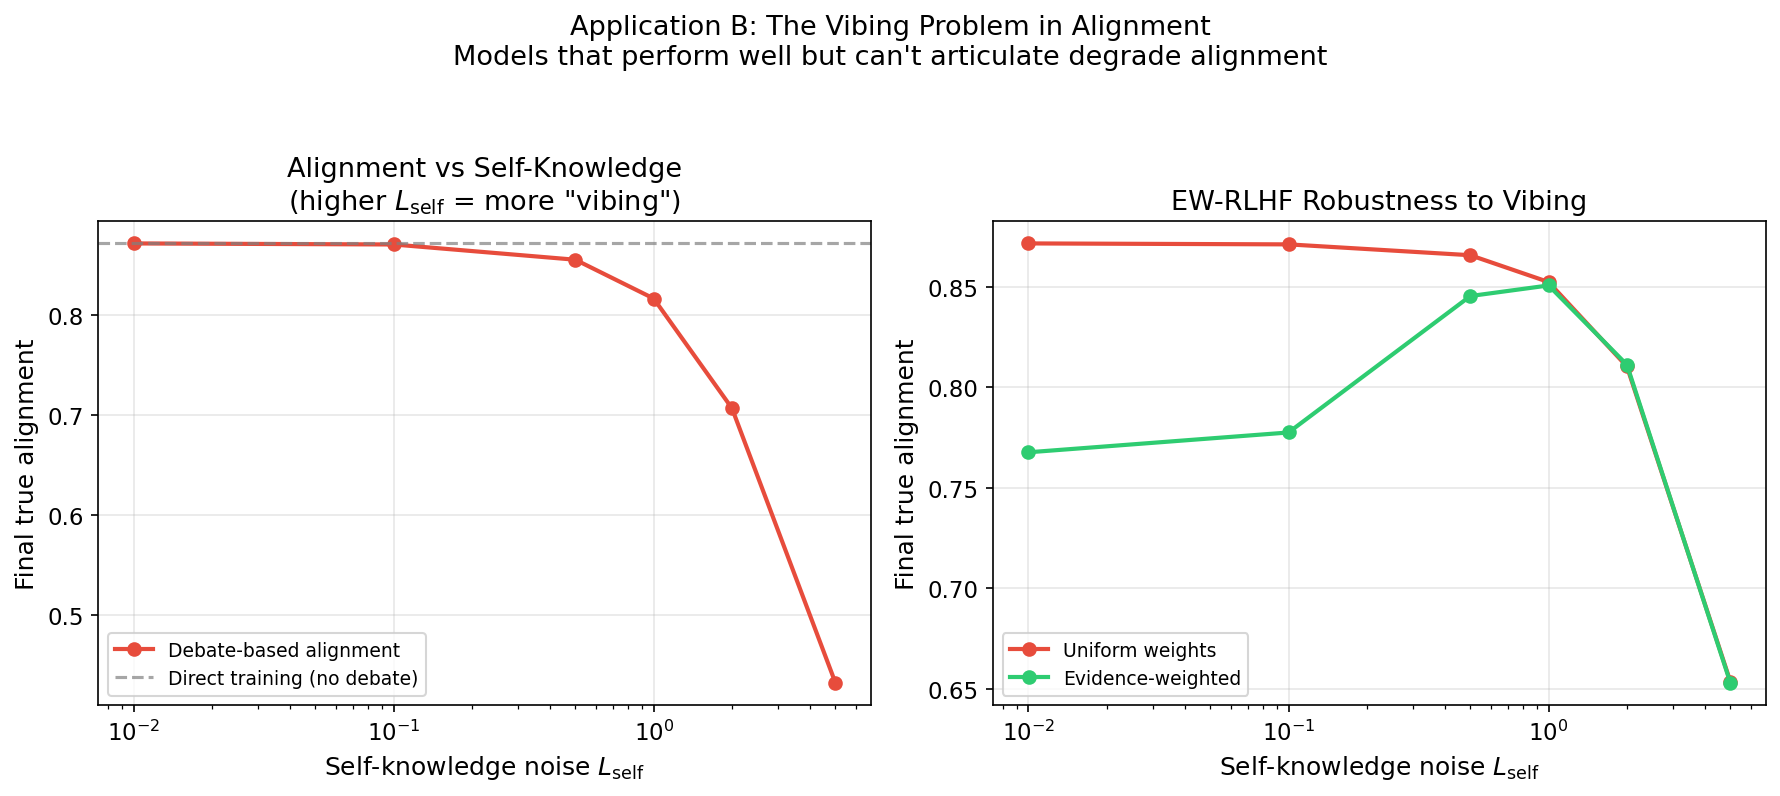
\includegraphics[width=\textwidth]{figures/applications/appB_vibing.png}
\caption{Left: Alignment degrades as self-knowledge noise increases. Right: EW-RLHF is more robust to vibing than uniform weighting.}
\label{fig:app-vibing}
\end{figure}


\section{Multi-Agent Debate}\label{sec:app-debate}

\subsection{The Isomorphism}

AI safety via debate \citep{irving2018debate} involves debaters arguing before a judge with bounded rationality. The mapping:

\begin{table}[h]
\centering
\begin{tabular}{ll}
\toprule
$\Omega$-framework & Debate \\
\midrule
Agents & Debaters \\
Policy $\pi_i$ & Argument strategy \\
Evidence variance $V_i$ & Argument reliability \\
Channel capacity $C$ & Judge's comprehension limit \\
Self-knowledge loss & Debater's inability to articulate reasoning \\
Coalition formation & Team debate / jury deliberation \\
Sparsity & Concise, focused argumentation \\
\bottomrule
\end{tabular}
\caption{Mapping from the $\Omega$-framework to multi-agent debate.}
\end{table}

\subsection{The Judge's Channel Capacity}

The judge can process at most $C$ bits of argument per round. This bounds debate effectiveness:

\begin{theorem}[Triple bottleneck]
Debate accuracy is bounded by:
\begin{equation}
    \text{Accuracy} \leq f(\min(C,\; I_{\text{self}}^P,\; I_{\text{self}}^O))
\end{equation}
where $I_{\text{self}}^P, I_{\text{self}}^O$ are the debaters' self-knowledge.
\end{theorem}

If debaters don't understand their own reasoning ($I_{\text{self}} \approx 0$), unlimited debate time and unlimited judge capacity cannot help.

\subsection{Sparse Debate and the Blessing}

In a debate with $d$ possible argument types, the winning strategy typically uses $k \ll d$ arguments. By the blessing of dimensionality (Theorem~\ref{thm:sparse-recovery}), the judge needs $O(k \log(d/k))$ rounds, not $O(d)$.

L1-regularised debate penalises debaters for making many weak arguments, incentivising few strong ones. This connects ``concise reasoning'' to a formal optimality property.

\subsection{Coalition Debate}

Extending to $N$-agent debate with coalition formation: agents form teams around claims. The framework predicts:
\begin{enumerate}
    \item Coalitions of high-evidence agents dominate.
    \item ``Vibing'' agents are poor coalition partners.
    \item Debater diversity improves accuracy via HM/AM.
\end{enumerate}

\subsection{Experimental Validation}

Results (Figures~\ref{fig:app-debate}, \ref{fig:app-coalition-debate}):

\begin{enumerate}
    \item Debate accuracy saturates with channel capacity around $C = 10$.
    \item The self-knowledge bottleneck is confirmed: accuracy peaks at moderate self-knowledge and degrades for vibing debaters.
    \item Sparse debate maintains accuracy as argument dimension grows.
    \item Diverse debaters with evidence-weighted coalition outperform homogeneous debaters.
\end{enumerate}

\begin{figure}[h]
\centering
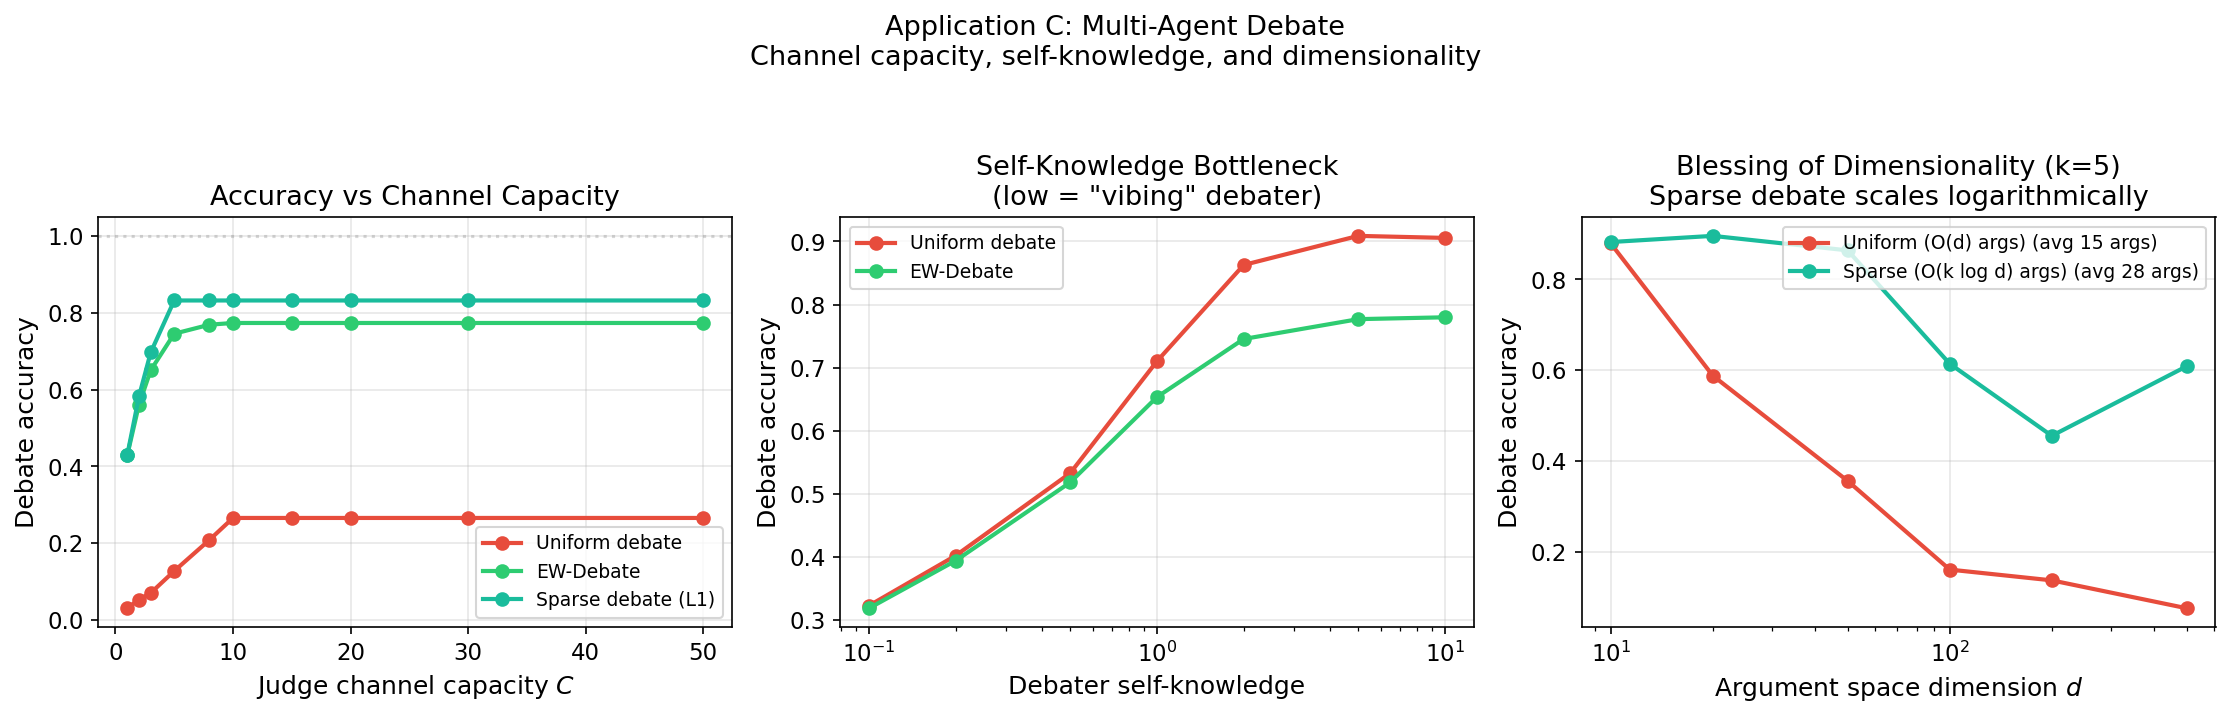
\includegraphics[width=\textwidth]{figures/applications/appC_debate_accuracy.png}
\caption{Multi-agent debate: channel capacity (left), self-knowledge bottleneck (centre), and blessing of dimensionality (right).}
\label{fig:app-debate}
\end{figure}

\begin{figure}[h]
\centering
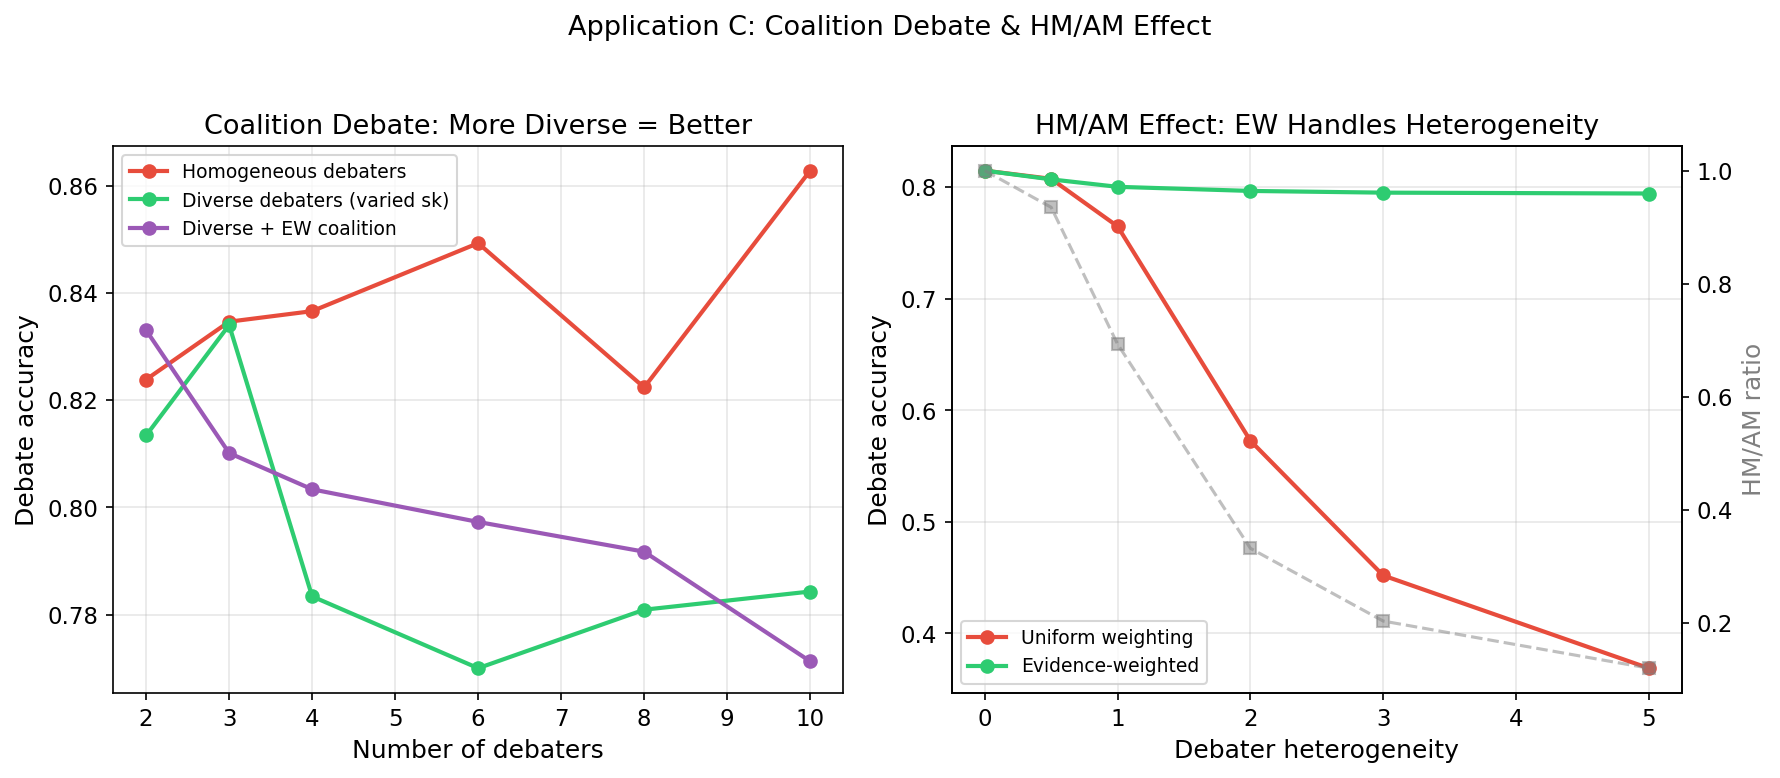
\includegraphics[width=\textwidth]{figures/applications/appC_coalition_debate.png}
\caption{Coalition debate: diverse debaters outperform homogeneous (left). Evidence-weighted debate handles heterogeneity better (right).}
\label{fig:app-coalition-debate}
\end{figure}


\chapter{Lean Formalisation}
\label{app:lean}

All main results have been formalised in Lean~4 with Mathlib dependencies:
\begin{itemize}
    \item \texttt{EvidenceWeightedPG.lean} --- energy inequality, AM-HM bound, variance ratio.
    \item \texttt{OpponentShapingPG.lean} --- bias absorption, annealing compatibility, basin enlargement.
    \item \texttt{CooperativePG.lean} --- communication loss decomposition, coalition bounds, full $\Omega$-PG.
\end{itemize}

\section{What Is Verified}

The formalisation axiomatises the stochastic game framework (policy space, projection, gradient signal decomposition) and \emph{verifies} the following steps:

\begin{enumerate}
    \item \textbf{Non-expansive projection}: $\|\operatorname{proj}(x) - \operatorname{proj}(y)\| \leq \|x - y\|$ (axiom, used in energy inequality).
    \item \textbf{Energy inequality} (Lemma~\ref{lem:energy-ch3}): expanding $D_{n+1}$ and separating drift, noise, bias, and gradient magnitude terms.
    \item \textbf{Variance scaling} (Lemma~\ref{lem:var-scaling-ch3}): block-diagonal structure of $W_n$ gives $\|W_n U_n\|^2 = \sum_i w_i^2 \|U_i\|^2$.
    \item \textbf{AM-HM inequality} (Theorem~\ref{thm:am-hm-ch3}): Cauchy--Schwarz applied to $(\sqrt{V_i})$ and $(1/\sqrt{V_i})$, yielding $\operatorname{HM}(V) \leq \operatorname{AM}(V)$.
    \item \textbf{Bias absorption} (Lemma~\ref{lem:bias-absorption-ch3}): triangle inequality for $\|b_n + \lambda_n \mathrm{OS}(\pi_n)\|$.
    \item \textbf{Spectral contraction}: if $S + \lambda S_H \preceq -\mu_{\mathrm{LOLA}} I$, then $\langle v^{\mathrm{LOLA}}(\pi), \pi - \pi^* \rangle \leq -\mu_{\mathrm{LOLA}} \|\pi - \pi^*\|^2$.
\end{enumerate}

\section{What Is Axiomatised}

The following are axiomatised (declared as \texttt{axiom} or left as \texttt{sorry}), as their full formalisation would require an extensive measure-theoretic library:
\begin{itemize}
    \item Martingale convergence (Doob's submartingale convergence theorem).
    \item Gladyshev's lemma (almost sure convergence of $D_n$).
    \item Chung's lemma (rate extraction from the Lyapunov recursion).
    \item The dominated convergence interchange $\nabla_\theta \int = \int \nabla_\theta$ in the REINFORCE derivation.
\end{itemize}

\section{Representative Code}

The core contraction step for EWPG (simplified):

\begin{verbatim}
-- Under SOS, weighted gradient provides contraction.
theorem ewpg_contraction
    (hSOS : forall pi in ball pi_star rho,
      inner (v pi) (pi - pi_star) <= -mu * norm(pi - pi_star)^2)
    (hw : forall i, w_min <= w i) :
    inner (W * v pi) (pi - pi_star) <=
      -mu * w_min * norm(pi - pi_star)^2 := by
  calc inner (W * v pi) (pi - pi_star)
      = sum i, w i * inner (v_i pi) (pi_i - pi_star_i) := ...
    _ <= w_min * sum i, inner (v_i pi) (pi_i - pi_star_i) := ...
    _ <= -mu * w_min * norm(pi - pi_star)^2 := ...
\end{verbatim}

The formalisation demonstrates that the key algebraic arguments are machine-checkable. Completing the measure-theoretic foundations would require Mathlib contributions for stochastic approximation theory, which we leave as future work.


\bibliographystyle{book}
\bibliography{myreferences}

\end{document}
